%=======================================================================
%  Relatório de Econometria e Análise de Intervenção
%  Modelagem de séries temporais diárias de Valor e Quantidade de propostas
%  Autor: Daniel Ramazzotte
%  Referência principal: "Projeção de Vendas — Definição de Modelo (v2)"
%  Compilar com: pdflatex/tectonic (2x, para referências cruzadas)
%=======================================================================
\documentclass[11pt,a4paper]{article}

\usepackage[utf8]{inputenc}
\usepackage[T1]{fontenc}
\usepackage[brazil]{babel}
\usepackage{lmodern}
\usepackage[a4paper,margin=2.5cm]{geometry}
\usepackage{amsmath,amssymb}
\usepackage{booktabs}
\usepackage{multirow}
\usepackage{graphicx}
\usepackage{float}
\usepackage{caption}
\usepackage{subcaption}
\usepackage{siunitx}
\usepackage{microtype}
\usepackage{pifont}
\usepackage[dvipsnames]{xcolor}
\usepackage[colorlinks=true,linkcolor=NavyBlue,citecolor=NavyBlue,urlcolor=NavyBlue]{hyperref}

\sisetup{output-decimal-marker={,},group-separator={.},group-minimum-digits=4}
\graphicspath{{img_sarima/}}
\captionsetup{font=small,labelfont=bf}
\emergencystretch=3em % relaxa o espaçamento para evitar overfull boxes
\Urlmuskip=0mu plus 1mu\relax

% --- Cabeçalho de título -------------------------------------------------
\title{\vspace{-1.2cm}\textbf{Previsão de Vendas Diárias de Propostas de Crédito:\\[3pt]
do AutoML à Econometria Interpretável}\\[6pt]
\large Construção da base, seleção experimental de modelos (TPOT $\rightarrow$ \emph{walk-forward})
e modelagem SARIMA com análise de intervenção de Box--Tiao}
\author{Daniel Ramazzotte\\[2pt]
\small Disciplina: Econometria e Análise de Intervenção}
\date{Julho de 2026}

\begin{document}
\maketitle

%========================================================================
\begin{abstract}
\noindent
Este trabalho aplica a metodologia clássica de Box--Jenkins, estendida pela análise de
intervenção de Box--Tiao e por testes de cointegração, à previsão diária de duas séries
operacionais de uma financeira de crédito: o \emph{valor} monetário e a \emph{quantidade} de
propostas processadas por dia útil. O objetivo é testar se um modelo \emph{branco} (interpretável)
do tipo SARIMA, com uma \emph{única especificação congelada}, consegue igualar ou superar o
sistema de \emph{AutoML} (TPOT) atualmente em produção, que é retreinado quase diariamente. As
séries são identificadas como $I(1)$ com sazonalidade semanal de dias úteis ($s=5$);
os dias atípicos (incidentes operacionais e vésperas de feriado) são tratados por funções de
transferência de intervenção em vez de descartados da estimação. A validação usa
\emph{walk-forward} de um passo à frente, sem vazamento, e o critério de seleção é o RMSPE ---
justificado por decompor o erro em viés e dispersão. Os principais resultados: (i) \textbf{não há
cointegração} confiável entre valor e quantidade, legitimando a modelagem separada; (ii) a
intervenção \textbf{descontamina o ajuste} --- o teste de Ljung--Box deixa de rejeitar a hipótese
de resíduos não-autocorrelacionados ($p$ de $\approx 0{,}01$ para $0{,}37$ e $0{,}63$); e (iii) o
SARIMA \textbf{iguala ou supera} a pipeline em produção no RMSPE nas duas séries, preservando
interpretabilidade estatística de cada componente.

\vspace{4pt}
\noindent\textbf{Palavras-chave:} SARIMA; análise de intervenção; Box--Tiao; cointegração;
RMSPE; \emph{walk-forward}; previsão de vendas.
\end{abstract}

%========================================================================
\section{Introdução}
\label{sec:intro}

A área de crédito precisa antecipar, todo dia útil, duas grandezas operacionais distintas para o
dia seguinte. A \textbf{quantidade} de propostas dimensiona a equipe e a fila de análise
(capacidade de atendimento); o \textbf{valor} monetário dimensiona capital, caixa e risco. Ambas
já são previstas em produção por um pipeline de \emph{AutoML} (TPOT) --- uma busca automatizada
entre milhares de combinações de \emph{features} e algoritmos de \emph{machine learning},
\emph{retreinado quase diariamente}. O pipeline é acurado, mas é uma \textbf{caixa-preta}: dele não
se lê ``quanto a fila pesa'' nem ``quanto um erro operacional custa'' na previsão, e o retreino
diário o torna caro e difícil de auditar.

\paragraph{O estudo em três atos.} Este trabalho percorre a evolução completa do sistema de
previsão:
\begin{enumerate}\setlength\itemsep{2pt}
\item \textbf{O baseline em produção} (Seção~\ref{sec:tpot}): a rotina diária de \emph{AutoML}
(TPOT), sua construção de base e engenharia de \emph{features} por defasagens, e seus limites
(caixa-preta, retreino diário).
\item \textbf{A seleção experimental} (Seção~\ref{sec:experimento}): um experimento controlado que
compara dezenas de candidatos (modelos simples, \emph{ensembles}, \emph{deep learning} e séries
temporais clássicas) sob \emph{walk-forward} alinhado ao histórico, com o objetivo de
\emph{substituir o TPOT por um modelo fixo, rápido e confiável}.
\item \textbf{A modelagem econométrica} (Seções~\ref{sec:sarima-modelo} em diante): o vencedor
interpretável --- um \textbf{SARIMA} com \textbf{análise de intervenção de Box--Tiao} --- é então
identificado, diagnosticado e estimado em detalhe.
\end{enumerate}

\paragraph{Pergunta de pesquisa.} Um modelo econométrico \emph{clássico} de séries temporais
(SARIMA), com estrutura interpretável e uma \emph{única} especificação fixa (não retreinada a cada
dia, apenas reestimada), consegue \emph{igualar ou superar} a pipeline TPOT em produção nas duas
séries que ela já prevê? Se o modelo branco vencer ou empatar, ganha-se interpretabilidade sem
sacrificar acurácia: coeficientes com significância estatística, tratamento transparente dos dias
atípicos (intervenção de Box--Tiao em vez de descarte cego) e um modelo auditável.

%========================================================================
\section{Dados e construção da base}
\label{sec:dados}

As propostas (etapa 16) são agregadas em frequência \textbf{diária}, apenas em \textbf{dias úteis}
(excluindo sábados, domingos e feriados nacionais via \texttt{workadays}). A ausência de feriados
na grade produz uma sazonalidade semanal regular de período $s = 5$. A Tabela~\ref{tab:base}
resume as duas séries-alvo.

\begin{table}[H]
\centering
\caption{Definição das séries-alvo. As duas têm o mesmo \emph{status}: cada uma recebe seleção de
ordem, intervenção, \emph{ranking} e modelo recomendado próprios.}
\label{tab:base}
\small
\begin{tabular}{@{}lll@{}}
\toprule
 & \textbf{Valor (R\$)} & \textbf{Quantidade} \\
\midrule
Definição & valor monetário processado no dia & n\textsuperscript{o} de propostas analisadas no dia \\
Papel     & série-alvo & série-alvo \\
Histórico & \multicolumn{2}{l}{$\approx$ 410 dias úteis (07/11/2024 $\rightarrow$ 01/07/2026)} \\
Janela \emph{walk-forward} & $N = 209$ & $N = 211$ \\
\bottomrule
\end{tabular}
\end{table}

Ambas exibem \textbf{nível que passeia} (não-estacionariedade), \textbf{sazonalidade semanal} e
\textbf{quedas pontuais} nos dias de erro operacional (Figura~\ref{fig:series}).

\begin{figure}[H]
\centering
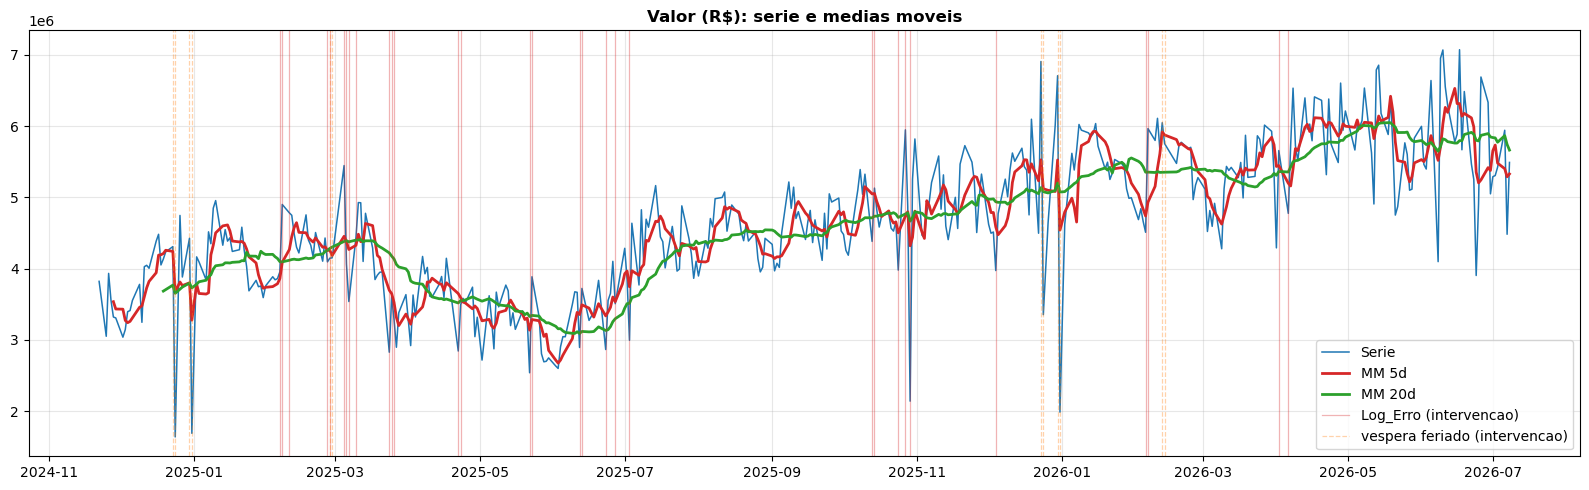
\includegraphics[width=0.84\linewidth]{valor_serie.png}\\[4pt]
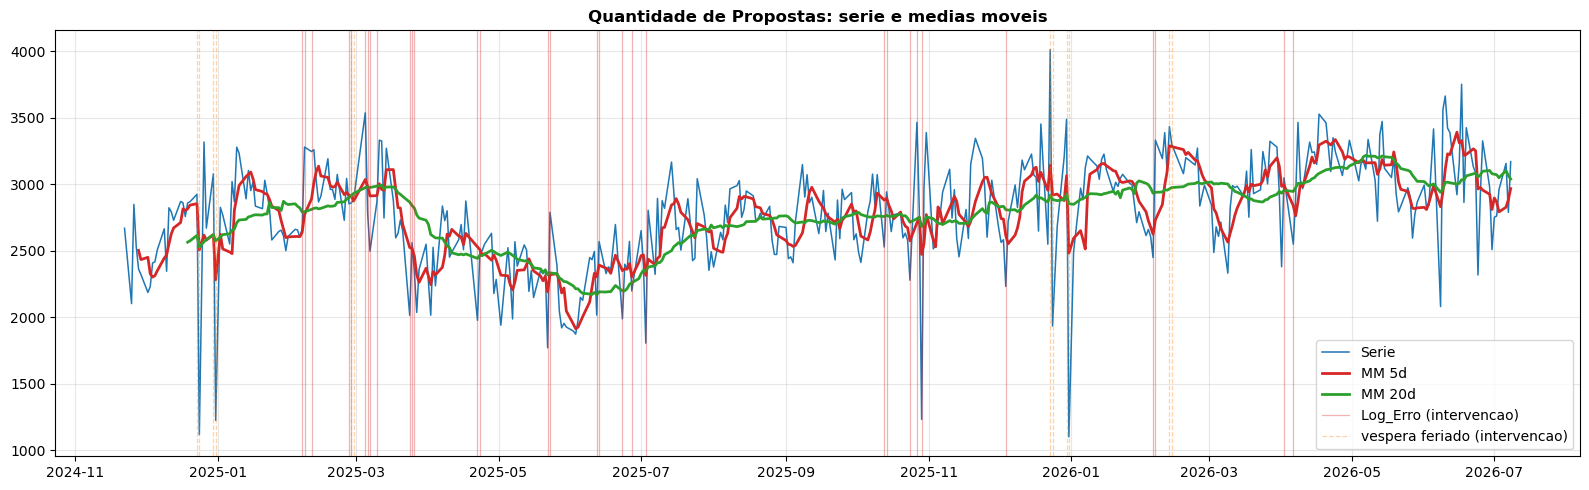
\includegraphics[width=0.84\linewidth]{qtd_serie.png}
\caption{Séries diárias de valor (topo) e quantidade (base), com médias móveis de 5 e 20 dias.
As linhas verticais marcam os dias de intervenção (incidentes e vésperas de feriado).}
\label{fig:series}
\end{figure}

%========================================================================
\section{O sistema em produção: AutoML diário (TPOT)}
\label{sec:tpot}

O ponto de partida --- e o \emph{benchmark} a bater --- é a rotina em produção
(\texttt{scripts/producao/projecoes\_qtd.py} e \texttt{projecoes\_valor.py}), que roda todo dia
útil e prevê o dia seguinte com um pipeline de \emph{AutoML} (TPOT).

\paragraph{Construção da base.} A cada execução, o script consulta o ClickHouse (propostas da
etapa 16, em janelas de 15 minutos) e agrega por dia; toma os \textbf{$\approx$ 45 dias úteis}
anteriores ao dia de referência (o último dia útil fechado). Os \textbf{dias atípicos}
(\texttt{Log\_Erro} $+$ vésperas de feriado) são removidos \emph{antes} de montar as
defasagens, para não contaminarem nem o alvo nem os \emph{lags} dos dias vizinhos.

\paragraph{Engenharia de \emph{features} (defasagens).} O modelo não é temporal por construção ---
a dinâmica é injetada como colunas de defasagem, mais o dia da semana:
\begin{itemize}\setlength\itemsep{1pt}
\item \textbf{Quantidade:} \texttt{dia\_semana}, \texttt{lag\_0}$=$valor de ontem,
\texttt{lag\_1..6}$=$quantidade dos 6 dias úteis anteriores. Alvo: quantidade.
\item \textbf{Valor:} \texttt{dia\_semana}, \texttt{lag\_0}$=$quantidade de ontem,
\texttt{lag\_1..6}$=$valor dos 6 dias anteriores, e \texttt{lag\_7}$=$\textbf{fila} de pagamento de
ontem (etapa 15, 2\textsuperscript{o} \emph{query}). Alvo: valor.
\end{itemize}

\paragraph{Busca AutoML e validação.} O TPOT faz busca evolutiva (\emph{60 gerações},
\emph{população 60}) sobre combinações de pré-processadores e regressores, otimizando um pipeline
para o alvo. A validação é um \textbf{teste de 1 dia} (a última observação): calcula-se o
\textbf{MAPE} e aceita-se o modelo se $1\% \le \text{MAPE} \le 5\%$; caso contrário, retreina-se
(até 4$\times$ na quantidade, 3$\times$ no valor). O pipeline aprovado é serializado em
\texttt{modelos/\{quantidade,valor\}/} e o mais recente é carregado para prever o próximo dia útil,
com o resultado registrado em \texttt{resultados/backup\_\{qtd,valor\}.xlsx}.

\paragraph{Limitações que motivam o estudo.} O TPOT é acurado, mas (i) é \textbf{caixa-preta} ---
a arquitetura empilhada não revela ``quanto a fila pesa'' ou ``quanto um erro custa''; (ii) é
\textbf{retreinado quase diariamente}, o que o torna caro, não-determinístico e difícil de
auditar; e (iii) valida-se em \textbf{um único ponto} por dia, uma medida ruidosa de qualidade.
Isso motiva buscar um modelo \emph{fixo, rápido e interpretável} que iguale seu desempenho.

%========================================================================
\section{Seleção experimental de um modelo substituto}
\label{sec:experimento}

O objetivo do experimento (notebooks \texttt{experimento\_qtd.ipynb} e
\texttt{experimento\_valor.ipynb}) é \textbf{substituir o TPOT por um modelo confiável e rápido},
comparando dezenas de candidatos sob um protocolo de avaliação honesto e idêntico para todos.

\paragraph{Protocolo \emph{walk-forward} alinhado ao histórico.} Cada candidato é avaliado com
\texttt{TimeSeriesSplit(test\_size=1, max\_train\_size=JANELA)} --- \textbf{um \emph{fold} por dia}
do \emph{backup}, retreinando na janela anterior e prevendo o próximo dia, sem jamais ver o futuro.
A janela de datas é ancorada na \emph{data mínima do backup}, para cobrir todo o período e comparar
\textbf{maçã-com-maçã} com a \textbf{Pipeline Antiga} (as previsões que o TPOT realmente fez em
produção). Todos os candidatos usam as \emph{features} da Seção~\ref{sec:tpot}, exceto os modelos
de série temporal, que aprendem a dinâmica diretamente.

\paragraph{Famílias de candidatos.} O experimento é organizado em partes:
\begin{itemize}\setlength\itemsep{1pt}
\item \textbf{Parte 1 --- modelos simples}: regressores com hiperparâmetros padrão (lineares,
árvores, \emph{gradient boosting}), um ponto de teste por dia.
\item \textbf{Parte 2 --- abordagens avançadas}: reproduzem, de forma transparente, o que o TPOT
faz --- seleção de variáveis (\texttt{SelectKBest}), \emph{tuning} (\texttt{RandomizedSearchCV}),
\emph{ensembles} (\texttt{Voting}/\texttt{Stacking}) e \emph{pipelines} com pré-processamento.
\item \textbf{Parte 3 --- \emph{deep learning} e séries temporais}: LSTM, CNN~1D e \emph{Transformer};
e modelos com dependência temporal explícita --- \textbf{Auto-ARIMA}, \textbf{Prophet} e
\textbf{NeuralProphet}. Também se avaliam \textbf{retrospectivamente} os próprios \emph{pipelines}
TPOT de produção (cada \texttt{.pkl}) nos mesmos \emph{folds}.
\end{itemize}

\paragraph{Exclusão de dias atípicos na avaliação.}
\label{sec:excluir}
Há uma distinção importante entre \emph{estimar} e \emph{avaliar}: os dias atípicos podem entrar no
treino (no SARIMA, via intervenção), mas são \textbf{removidos do \emph{ranking}}. Manter um dia de
falha operacional na comparação penalizaria (ou premiaria) os modelos por ruído operacional, não
por capacidade preditiva, distorcendo o MAPE/RMSPE. A remoção (\texttt{mask\_dias\_excluir}) segue
três critérios: (i) \textbf{Log de Erro} --- o dia do incidente e os $n-1$ dias úteis seguintes
(coluna \emph{impacto}, pois a fila represada ``vaza'' para os dias seguintes); (ii) \textbf{véspera
de feriado} (Natal, Ano-Novo, Carnaval e o dia anterior); (iii) \textbf{outliers manuais}
pontuais. A comparação usa as previsões \emph{cruas} (sem correção de viés), sobre a mesma base
comum de datas.

\paragraph{Critério de seleção --- por que RMSPE.} O \emph{ranking} é ordenado por \textbf{RMSPE},
porque ele decompõe o erro em viés e dispersão:
\begin{equation}
\text{RMSPE} = \sqrt{\frac{1}{N}\sum_{t=1}^{N}\!\left(\frac{y_t-\hat y_t}{y_t}\right)^{\!2}},
\qquad
\underbrace{\text{RMSPE}^2}_{\text{erro total}} = \underbrace{\text{Viés}\%^2}_{\text{descentramento}} + \underbrace{\text{Dispersão}\%^2}_{\text{espalhamento}}.
\label{eq:rmspe}
\end{equation}
Se o erro percentual fosse igual todo dia (dispersão $=0$), teríamos RMSPE $=$ MAPE; quanto maior a
dispersão, mais o RMSPE se afasta do MAPE. Exemplo: para APEs $(0,0,6,6)$, MAPE $=3$ e dispersão
$=3$, logo RMSPE $=\sqrt{9+9}=4{,}24\%$. Assim o RMSPE \textbf{penaliza \emph{outliers}} mais que o
MAPE e captura o \emph{trade-off viés $\times$ variância}. As demais métricas completam o retrato:
MAPE (erro típico), $R^2$, Viés/MPE (erro sistemático), DP Erro, Máx.\% (pior dia) e as frações de
dias com erro $<5\%/<10\%$. Meta: MAPE $\le 5\%$ (ideal), $\le 10\%$ (aceitável).

\paragraph{Do experimento à modelagem SARIMA.} O experimento mostrou que \emph{nenhum} enriquecimento
de \emph{features} ou família de ML supera de forma consistente e interpretável os modelos de
\textbf{série temporal clássica}: entre os candidatos que \emph{igualam ou batem} a Pipeline
Antiga, o \textbf{SARIMA} é o mais parcimonioso e o único totalmente auditável. Ele é, portanto,
promovido de \emph{benchmark} a \textbf{modelo recomendado} --- e o restante do relatório o
identifica, trata seus dias atípicos por intervenção e o estima e valida em detalhe.

%========================================================================
\section{Modelagem SARIMA: especificação, identificação e intervenção}
\label{sec:sarima-modelo}

\subsection{O modelo SARIMA/SARIMAX}
\label{sec:sarima}

Seja $B$ o operador de defasagem ($B^k y_t = y_{t-k}$). Um modelo
$\text{SARIMA}(p,d,q)(P,D,Q)_s$ com regressores exógenos (SARIMAX) escreve-se como uma
\textbf{regressão com erros SARIMA}:
\begin{equation}
y_t = \boldsymbol{\beta}'\mathbf{X}_t + \eta_t,
\qquad
\phi(B)\,\Phi(B^s)\,(1-B)^d(1-B^s)^D\,\eta_t = \theta(B)\,\Theta(B^s)\,\varepsilon_t,
\label{eq:sarimax}
\end{equation}
onde $\mathbf{X}_t$ reúne os regressores de intervenção (Seção~\ref{sec:interv}),
$\varepsilon_t \sim \text{RB}(0,\sigma^2)$, e $\phi,\theta,\Phi,\Theta$ são, respectivamente, os
polinômios autorregressivo e de média móvel não-sazonais e sazonais. Nesta aplicação $s=5$ e, como
se verá, $d=1,\ D=0$. Os dois modelos escolhidos são \textbf{SARIMA univariados} (não usam
covariável de negócio): os únicos regressores em $\mathbf{X}_t$ são as \emph{dummies} de
intervenção.

\subsection{Identificação: estacionariedade e ordem}
\label{sec:ident}

A identificação segue Box--Jenkins: (i) \textbf{estacionariedade} por ADF e KPSS; (ii) inspeção de
\textbf{ACF/PACF} em nível e na primeira diferença; (iii) \textbf{decomposição STL} (período 5)
para separar tendência, sazonal e resíduo. A ordem $(p,d,q)(P,D,Q)_5$ é escolhida por
\texttt{auto\_arima} (busca \emph{stepwise} minimizando o AIC), \emph{uma única vez}, sobre a série
inteira --- um vazamento \emph{leve e restrito à especificação}; os \textbf{coeficientes}, porém,
são reestimados honestamente a cada dia do \emph{walk-forward} (MLE via filtro de Kalman, só com o
passado --- Seção~\ref{sec:experimento}).

\subsection{Análise de intervenção (Box--Tiao)}
\label{sec:interv}

Dias atípicos --- incidentes operacionais registrados no \texttt{Log\_Erro} e vésperas de
Natal/Ano-Novo/Carnaval --- produzem \emph{spikes} que, se ignorados, contaminam a estimação de
$\phi,\theta,\Phi,\Theta$. Em vez de descartar esses dias da estimação, adota-se o \textbf{modelo
de intervenção de Box--Tiao}: cada evento entra como um regressor determinístico cuja resposta
dinâmica é uma \emph{função de transferência} aplicada a um indicador de pulso
\begin{equation}
P_t = \mathbb{1}[\,t \in \mathcal{D}_E\,],
\qquad
y_t = \frac{\omega(B)}{\delta(B)}\,B^{b}\,P_t \;+\; N_t,
\label{eq:boxtiao}
\end{equation}
onde $\mathcal{D}_E$ é o conjunto de datas do evento $E$, $N_t$ é o ruído SARIMA de
\eqref{eq:sarimax}, e $\tfrac{\omega(B)}{\delta(B)}B^{b}$ controla magnitude, atraso ($b$) e
persistência do efeito. Teoricamente, erros operacionais são \emph{impulsos} (não deixam impacto
permanente na série). As formas funcionais testadas por evento são casos particulares de
\eqref{eq:boxtiao}, resumidas na Tabela~\ref{tab:transfer}.

\begin{table}[H]
\centering
\caption{Famílias de função de intervenção testadas. O fator $\delta \in (0,1)$ controla a
velocidade do decaimento; $d_0<\dots<d_{n-1}$ são os dias úteis afetados por um evento de duração
$n$. A forma vencedora de cada evento é a de coeficiente(s) significativo(s) ($p<0{,}05$) e menor
AIC; sem nenhum significativo $\to$ ``não signif.''; empate $\to$ a mais simples.}
\label{tab:transfer}
\small
\renewcommand{\arraystretch}{1.45}
\begin{tabular}{@{}llp{5.2cm}@{}}
\toprule
\textbf{Forma} & \textbf{Regressor} & \textbf{Interpretação} \\
\midrule
Abrupto        & $x_t = P_t$ & choque constante nos dias de impacto, retorno abrupto a zero \\
Gradual        & $x_t = \tfrac{n-k}{n},\ t=d_k$ & rampa linear decrescente ($1$ no 1\textsuperscript{o} dia $\to 1/n$ no último) \\
Rebote (2 reg.)& $x^{(1)}_t=\mathbb{1}[t=d_0],\ x^{(2)}_t=\mathbb{1}[t\in\{d_1,\dots\}]$ & queda no 1\textsuperscript{o} dia + recuperação (sinais opostos) do \emph{backlog} \\
Transf.\ g     & $x_t=\delta x_{t-1}+P_t$ & choque temporário com decaimento geométrico \\
Transf.\ b     & $x_t=\delta x_{t-1}+P_{t-1}$ & igual ao \emph{g}, com atraso de um dia \\
Transf.\ c     & $x_t=\sum_{\tau\le t}P_\tau$ & degrau permanente (mudança de patamar) \\
Transf.\ e (2) & $x^{(1)}_t=P_t,\ x^{(2)}_t=\delta x^{(2)}_{t-1}+P_t$ & pulso imediato $+$ cauda que decai \\
Transf.\ d (2) & $x^{(1)}_t=\delta x^{(1)}_{t-1}+P_t,\ x^{(2)}_t=\sum_{\tau\le t}P_\tau$ & transitório que decai $+$ degrau permanente \\
Transf.\ f     & $x_t=\sum_{\tau\le t}v_\tau,\ v_\tau=\delta v_{\tau-1}+P_\tau$ & convergência suave a um novo patamar \\
\bottomrule
\end{tabular}
\end{table}

\noindent
Cada \textbf{tipo} de dia atípico é classificado de forma \emph{independente} por série: as
vésperas de feriado são separadas em ``dia anterior à véspera'' (D-1) e ``véspera'' propriamente, e
cada uma --- assim como cada incidente do \texttt{Log\_Erro} --- pode receber uma forma diferente
no valor e na quantidade. A intervenção \textbf{mantém} os dias especiais no treino (necessário
para estimar o efeito), mas nos dias de avaliação (normais) as \emph{dummies} valem zero. Assim,
os coeficientes AR/MA descrevem a \emph{dinâmica normal} da série, e cada choque atípico recebe um
coeficiente e um $p$-valor próprios --- exatamente o que a caixa-preta não oferece.

\subsection{Cointegração}
\label{sec:coint}

Como valor e quantidade parecem ``andar juntas'', testa-se se há \textbf{equilíbrio de longo
prazo} entre elas. Se forem cointegradas com vetor $(1,-\beta)$, o \emph{ticket médio}
$(\text{valor}/\text{qtd})$ seria estacionário. Aplicam-se \textbf{Engle--Granger} e
\textbf{Johansen} (traço) sobre os níveis, com seleção prévia do \emph{lag} do VAR por critério de
informação, mais o ADF do \emph{ticket} médio e o ADF com tendência (\texttt{ct}) para descartar
\emph{trend-stationarity}. Antes dos testes, remove-se dos níveis o efeito de \emph{pulso} dos dias
atípicos. O teste decide se as séries devem ser modeladas \emph{juntas} (VECM/ARDL) ou
\emph{separadamente}.

%========================================================================
\section{Resultados}
\label{sec:result}

\subsection{Identificação e estacionariedade}
\label{sec:res-ident}

A ACF em nível decai lentamente nas duas séries (não-estacionariedade), justificando $d=1$; na
primeira diferença surge um pico negativo no \emph{lag} 1 --- assinatura de \textbf{MA(1)}
(Figura~\ref{fig:acf}). A \textbf{decomposição STL} (período 5) confirma o padrão nas duas séries
(Figuras~\ref{fig:stl-valor} e~\ref{fig:stl-qtd}): \textbf{tendência} suave de médio prazo,
\textbf{sazonalidade semanal} clara e \textbf{resíduo} com \emph{spikes} concentrados nos dias
atípicos (que a intervenção trata). A ordem selecionada foi $\text{SARIMA}(0,1,1)(0,0,1)_5$ para o
valor e $(0,1,1)(0,0,2)_5$ para a quantidade.

\begin{figure}[H]
\centering
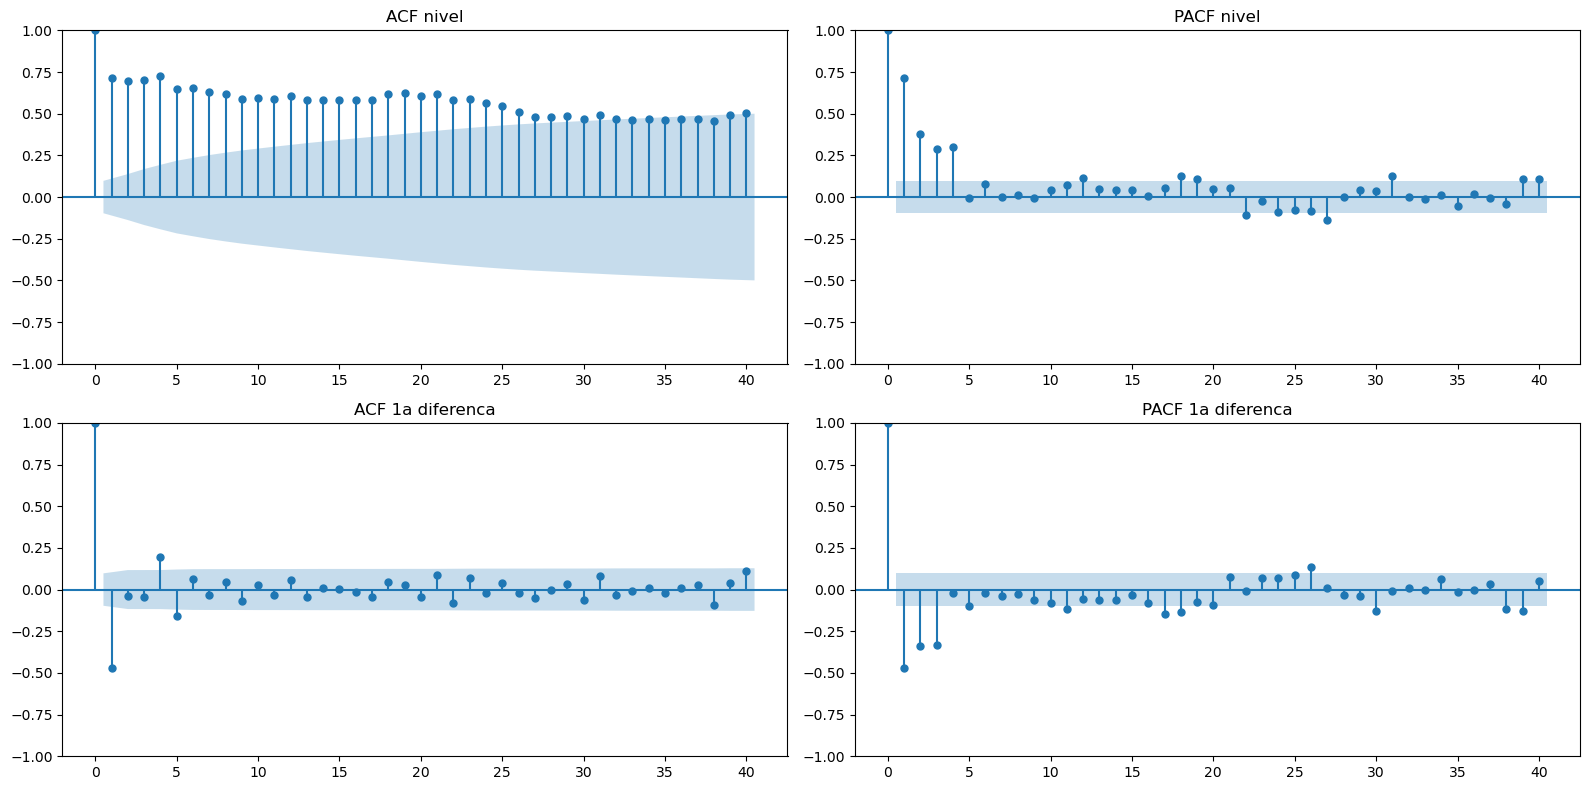
\includegraphics[width=0.8\linewidth]{valor_acf.png}
\caption{ACF/PACF do valor: nível decai lentamente ($I(1)$); a 1\textsuperscript{a} diferença
apresenta corte no \emph{lag} 1, sugerindo MA(1). Padrão análogo na quantidade.}
\label{fig:acf}
\end{figure}

\begin{figure}[H]
\centering
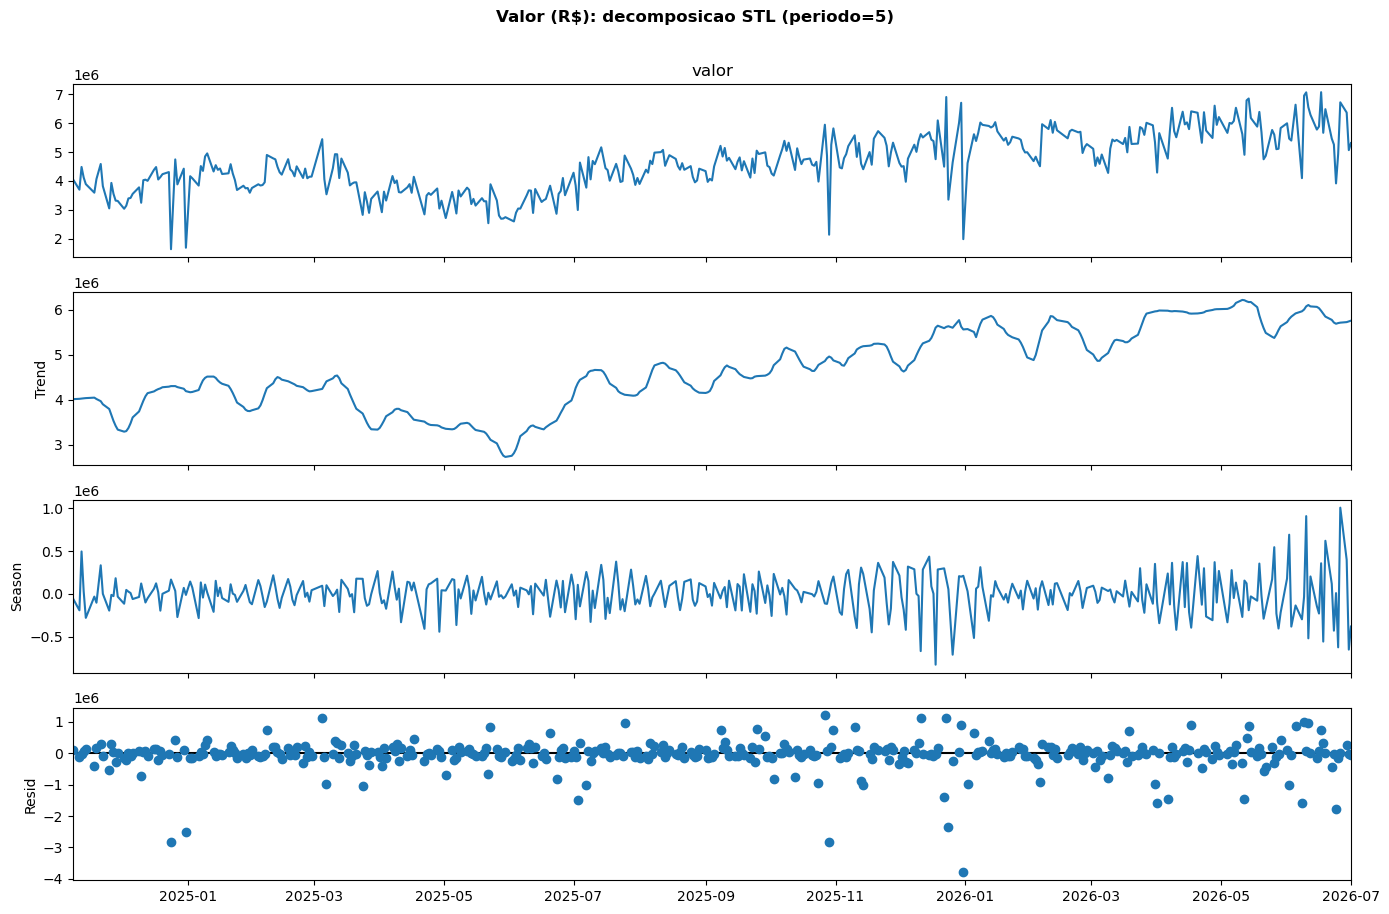
\includegraphics[width=0.86\linewidth]{stl_valor.png}
\caption{Decomposição STL (período 5) da série de \textbf{valor}: observado, tendência, sazonal
semanal e resíduo. A tendência sobe ao longo de 2025--2026; o resíduo concentra os \emph{spikes}
nos dias atípicos.}
\label{fig:stl-valor}
\end{figure}

\begin{figure}[H]
\centering
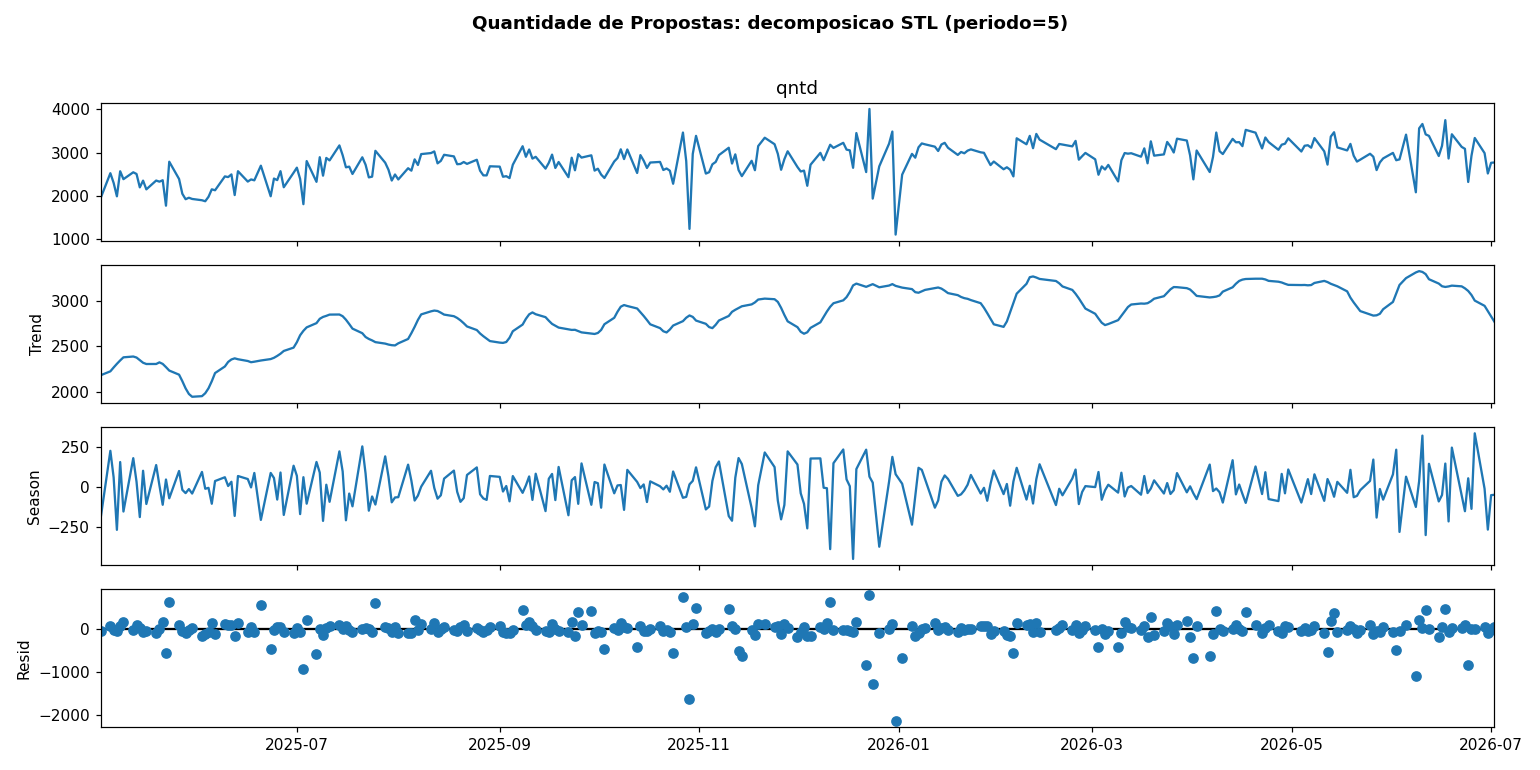
\includegraphics[width=0.86\linewidth]{stl_qtd.png}
\caption{Decomposição STL (período 5) da série de \textbf{quantidade}: mesmo padrão (tendência
$+$ sazonal semanal $+$ resíduo com \emph{spikes}), com histórico ligeiramente mais curto.}
\label{fig:stl-qtd}
\end{figure}

\subsection{Cointegração: não há equilíbrio de longo prazo}
\label{sec:res-coint}

Após remover o pulso dos dias atípicos, Engle--Granger \textbf{não rejeita} a ausência de
cointegração (estatística $=-0{,}60$, $p=0{,}956$) e o ADF do \emph{ticket} médio indica erro de
equilíbrio não-estacionário ($p=0{,}790$) --- Tabela~\ref{tab:coint}. O Johansen sem tendência
aponta 0 relações; com tendência determinística aponta 2, mas isso coincide com a
\emph{trend-stationarity} detectada pelo ADF-\texttt{ct}, ou seja, \emph{não} é cointegração
genuína. A relação estimada foi $\text{valor}=-1{.}536{.}713 + 2{.}220{,}46\cdot\text{qtd}$
($\beta \approx$ \emph{ticket} médio), mas seu resíduo \textbf{deriva} ao longo do tempo
(Figura~\ref{fig:coint}).

\begin{table}[H]
\centering
\caption{Testes de raiz unitária e cointegração (níveis ajustados para intervenção).}
\label{tab:coint}
\small
\begin{tabular}{@{}lccl@{}}
\toprule
Teste & Valor & Quantidade & Leitura \\
\midrule
ADF nível              & $p=0{,}060$ & $p=0{,}0005$ & valor $I(1)$ · qtd $I(0)$ (ordens mistas) \\
ADF 1\textsuperscript{a} dif. & $p=0{,}000$ & $p=0{,}000$ & ambas estacionárias diferenciadas \\
ADF-\texttt{ct}        & $p=0{,}0004$ & $p=0{,}0003$ & ambas \emph{trend-stationary} \\
Engle--Granger ($-0{,}60$) & \multicolumn{2}{c}{$p=0{,}956$} & \textbf{não rejeita} $\to$ sem cointegração \\
ADF do \emph{ticket} médio & \multicolumn{2}{c}{$p=0{,}790$} & erro de equilíbrio não-estacionário \\
\midrule
ARDL \emph{bounds} (caso III) & $F=2{,}34$ & $F=2{,}66$ & $F<$\,I(0)$_{5\%}{=}3{,}80$ $\to$ \textbf{não rejeita} \\
\bottomrule
\end{tabular}
\end{table}

\begin{figure}[H]
\centering
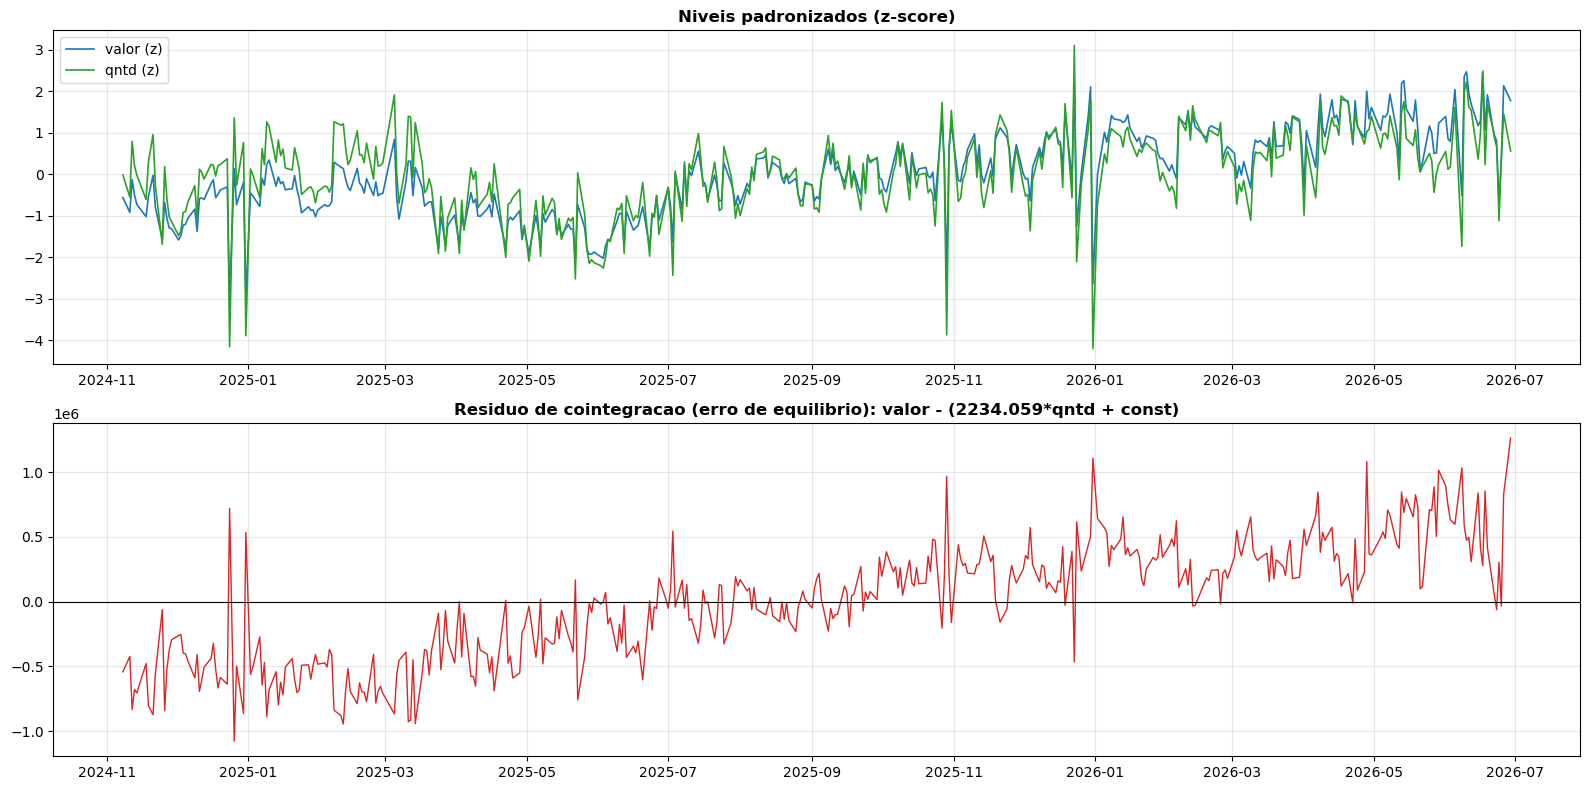
\includegraphics[width=0.8\linewidth]{coint.png}
\caption{Superior: valor e quantidade padronizados ($z$-score), dias atípicos ajustados em
vermelho. Inferior: resíduo de Engle--Granger --- \textbf{deriva} em vez de oscilar em torno de
zero, evidência visual da ausência de cointegração.}
\label{fig:coint}
\end{figure}

\paragraph{\emph{Follow-up} formal (ARDL).} Como as ordens de integração são \textbf{mistas}
$I(0)/I(1)$, o teste apropriado dispensa a pré-classificação em $I(1)$: o \textbf{teste de limites}
de Pesaran--Shin--Smith (\emph{bounds test}), que verifica a existência de uma \emph{relação de
nível}. Nas duas direções a estatística $F$ ($2{,}34$ para valor$|$qtd; $2{,}66$ para qtd$|$valor)
fica \textbf{abaixo do limite inferior} $I(0)$ a 5\% ($3{,}80$) --- \emph{não} se rejeita a ausência
de relação de nível, \textbf{confirmando} Engle--Granger e Johansen (Tabela~\ref{tab:coint}).

\subsubsection*{Por que a rejeição faz sentido, e como (não) modelar as séries juntas}
\label{sec:res-joint}

À primeira vista valor e quantidade ``andam juntas'' e a tentação é modelá-las conjuntamente. O
ponto é que \textbf{co-movimento contemporâneo $\neq$ cointegração}. Cointegração descreve um
\emph{equilíbrio de longo prazo}: um desvio entre as séries hoje é \emph{corrigido ao longo dos
dias} (mecanismo de correção de erro) --- um fenômeno \emph{defasado}. A relação valor--quantidade,
porém, é quase a identidade contábil \emph{contemporânea} $\text{valor}_t \approx \bar{t}_t \cdot
\text{qtd}_t$ (com $\bar{t}$ = \emph{ticket} médio do dia): mais propostas hoje $\to$ mais valor
\emph{hoje}, no mesmo dia, sem desequilíbrio que leve dias para se dissipar. Somando-se a isso que o
ADF-\texttt{ct} aponta as séries como \emph{trend-stationary} (próximas de $I(0)$), e que
cointegração --- definida apenas para séries $I(1)$ --- torna-se \emph{inaplicável}, a rejeição é o
resultado \textbf{esperado}, não um fracasso: ela só descarta a família VECM/correção de erro.

Rejeitar cointegração não impede modelagem conjunta --- muda apenas \emph{qual} modelo é apropriado.
Três alternativas foram testadas no \textbf{mesmo walk-forward 1-passo e nas mesmas datas} do
\emph{ranking} univariado (contraste controlado, todas sem \emph{dummies} de intervenção):
\begin{enumerate}\setlength\itemsep{1pt}
\item \textbf{(a) Decomposição por ticket} --- $\text{valor}=\text{qtd}\times\text{ticket}$:
prevê-se qtd e \emph{ticket} $(=\text{valor}/\text{qtd})$ por SARIMA e recompõe-se $\hat v=\hat
q\cdot\hat t$. Usa a identidade estrutural, mas \emph{exige prever qtd primeiro} (sistema
encadeado); só se aplica ao valor.
\item \textbf{(b) SUR bivariado} --- duas equações com regressores próprios defasados $+$
\emph{dummies} de dia-da-semana, estimadas em conjunto (FGLS de Zellner) com erros correlacionados.
\item \textbf{(c) VAR em diferenças} --- o modelo conjunto \emph{clássico quando não há
cointegração} (VAR nas 1\textsuperscript{as} diferenças, não VECM), com \emph{dummies} semanais como
exógenas.
\item \textbf{(d) ARDL encadeado} --- regressão ARDL de uma série sobre \emph{lags} da outra, com o
termo contemporâneo substituído pela previsão univariada da outra série (sem vazamento); a
contraparte \emph{preditiva} do teste de limites ARDL acima.
\end{enumerate}

A Tabela~\ref{tab:joint} traz o resultado. \textbf{O SARIMA univariado é o mais adequado.} Na
quantidade ele vence na frente (RMSPE 9,07\% contra 9,24\% do ARDL, 9,49\% do VAR e 10,80\% do SUR).
No valor, \emph{ticket} e \emph{ARDL encadeado} apenas \emph{empatam} (9,44\% e 9,51\% vs.\ 9,58\%,
$\approx 0{,}1$ p.p., dentro do ruído amostral) --- e nem são modelos de dinâmica conjunta: usam a
identidade estrutural e ainda precisam prever a quantidade antes ($\hat q$). Já \textbf{SUR e VAR
pioram} nas duas séries. O motivo confirma a
leitura da cointegração: o elo forte é \emph{contemporâneo} e, portanto, \emph{inutilizável} para
prever D+1 (não se conhece o qtd de amanhã ao prever o valor); resta o elo \emph{defasado}, fraco,
cujos termos cruzados só adicionam \textbf{variância} sem reduzir viés. Sem correção de erro
(i.e.\ sem cointegração), a informação cruzada não carrega conteúdo preditivo --- apenas ruído.

\begin{table}[H]
\centering
\caption{Modelagem conjunta vs.\ univariada --- walk-forward 1-passo, mesmas janelas (sem
intervenção). Menor RMSPE por série em negrito.}
\label{tab:joint}
\small
\begin{tabular}{@{}llccc@{}}
\toprule
Série & Modelo & RMSPE (\%) & MAPE (\%) & $R^2$ \\
\midrule
\multirow{5}{*}{Valor ($N{=}209$)}
 & \textbf{(a) Ticket} $\hat q\cdot\hat t$ & \textbf{9,44}  & 7,51 & 0,744 \\
 & (d) ARDL valor$\leftarrow$qtd            & 9,51           & 7,47 & 0,743 \\
 & SARIMA univariado                        & 9,58           & 7,71 & 0,730 \\
 & (c) VAR em diferenças                    & 9,89           & 7,75 & 0,701 \\
 & (b) SUR bivariado                        & 11,84          & 9,24 & 0,555 \\
\midrule
\multirow{4}{*}{Qtd.\ ($N{=}211$)}
 & \textbf{SARIMA univariado}               & \textbf{9,07}  & 7,32 & 0,399 \\
 & (d) ARDL qtd$\leftarrow$valor            & 9,24           & 7,56 & 0,372 \\
 & (c) VAR em diferenças                    & 9,49           & 7,31 & 0,335 \\
 & (b) SUR bivariado                        & 10,80          & 8,62 & 0,102 \\
\bottomrule
\end{tabular}
\end{table}

\noindent\textbf{Consequência metodológica:} como o erro de equilíbrio não reverte à média, o teste
de limites ARDL \emph{não rejeita} a ausência de relação de nível e \emph{nenhum} modelo conjunto
supera o univariado, \emph{modelam-se as séries separadamente} (SARIMA univariado $+$ intervenção).
As alternativas conjuntas ou empatam (\emph{ticket}/ARDL, estruturais e encadeados) ou pioram
(SUR/VAR). O \emph{follow-up} formal apropriado ao caráter misto $I(0)/I(1)$ é justamente o ARDL
(Pesaran--Shin--Smith), não o VECM --- e foi ele que fechou o argumento.

\subsection{Intervenção: classificação por evento e descontaminação do ajuste}
\label{sec:res-interv}

No modelo congelado de produção, \textbf{23 janelas de evento} foram classificadas em cada série
--- os 17 incidentes operacionais do \texttt{Log\_Erro} mais 6 janelas de véspera de feriado (o
``dia anterior'' D-1 e a ``véspera'', para Natal, Ano-Novo e Carnaval). A escolha da forma
vencedora é feita \emph{por série de forma independente}; a Tabela~\ref{tab:efeitos} resume a
distribuição das formas, a Figura~\ref{fig:interv} traz a \textbf{magnitude do efeito} evento a
evento, e a Figura~\ref{fig:interv-timeline} mostra os \textbf{eventos ao longo do tempo} sobre as
séries.

\begin{table}[H]
\centering
\caption{Distribuição das formas de intervenção escolhidas (função vencedora por AIC), por série
--- fonte: \texttt{config/modelo\_sarima\_producao.json}. As 23 janelas incluem os 17 incidentes
do \texttt{Log\_Erro} e 6 janelas de véspera.}
\label{tab:efeitos}
\small
\begin{tabular}{@{}lcc@{}}
\toprule
Forma de intervenção & \textbf{Valor} ($n$) & \textbf{Quantidade} ($n$) \\
\midrule
Abrupto (choque pontual)          & 5 & 3 \\
Gradual (rampa decrescente)       & 5 & 0 \\
Rebote (queda $+$ recuperação)    & 2 & 0 \\
\emph{b} (geom.\ com atraso 1 dia)& 3 & 4 \\
\emph{c} (degrau permanente)      & 0 & 3 \\
\emph{e} (pulso $+$ cauda)        & 3 & 2 \\
\emph{f} (patamar suave)          & 1 & 2 \\
\emph{g} (decaimento geométrico)  & 1 & 1 \\
Não signif.\ (descartado)         & 3 & 8 \\
\midrule
\textbf{Total}                    & \textbf{23} & \textbf{23} \\
\bottomrule
\end{tabular}
\end{table}

Dois padrões chamam a atenção. Primeiro, \textbf{muitos incidentes afetam o valor mas não a
quantidade}: são 8/23 janelas ``não signif.'' na quantidade contra apenas 3/23 no valor --- uma
parada operacional muda o \emph{quanto} é processado sem necessariamente mudar \emph{quantas}
propostas entram. Segundo, predominam formas com \textbf{decaimento/cauda} (\emph{b}, \emph{g},
\emph{e}, \emph{f}) em vez do choque puramente abrupto: o efeito de um erro não some de um dia para
o outro --- há \emph{backlog} processado nos dias seguintes. As vésperas seguem padrão próprio: o
dia anterior (D-1) é um pulso com cauda (\emph{e}, $\delta=0{,}1$) nas duas séries, enquanto a
véspera de Natal e de Ano-Novo é um choque \textbf{abrupto}; o Carnaval difere entre séries.

\begin{figure}[H]
\centering
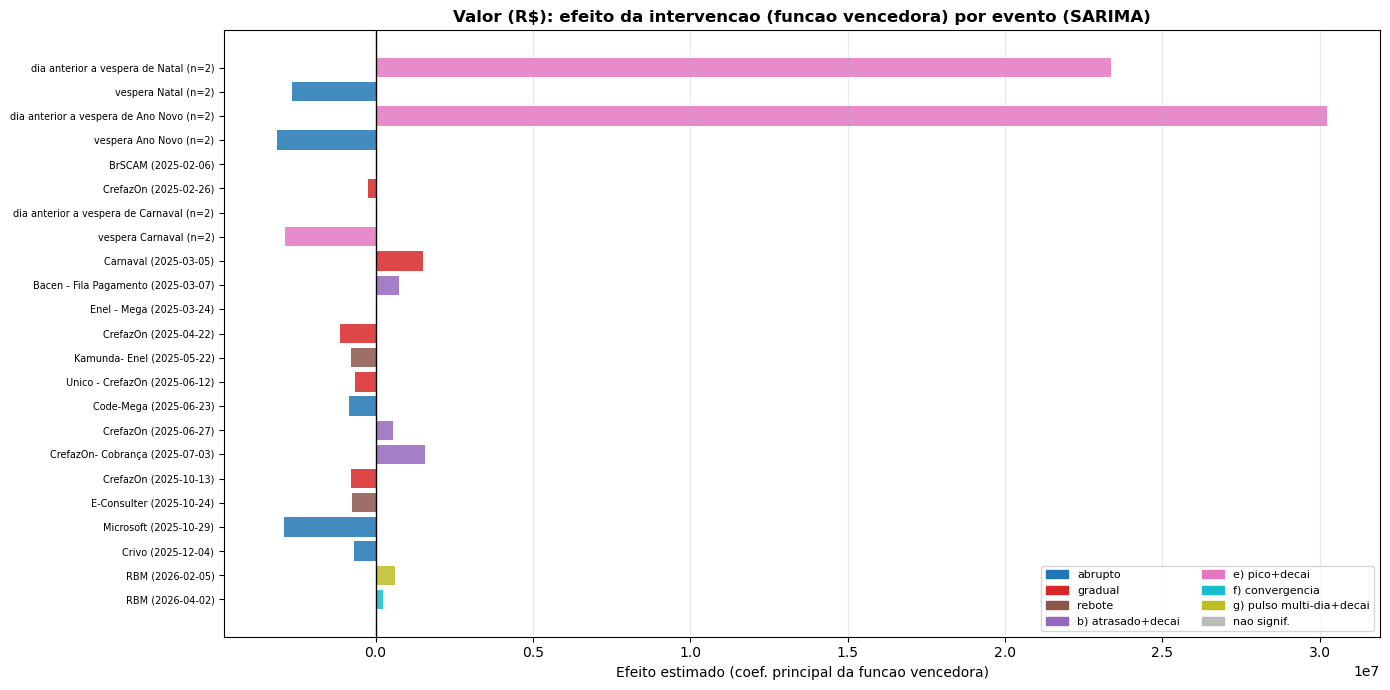
\includegraphics[width=0.99\linewidth]{interv_mag_valor.png}\\[3pt]
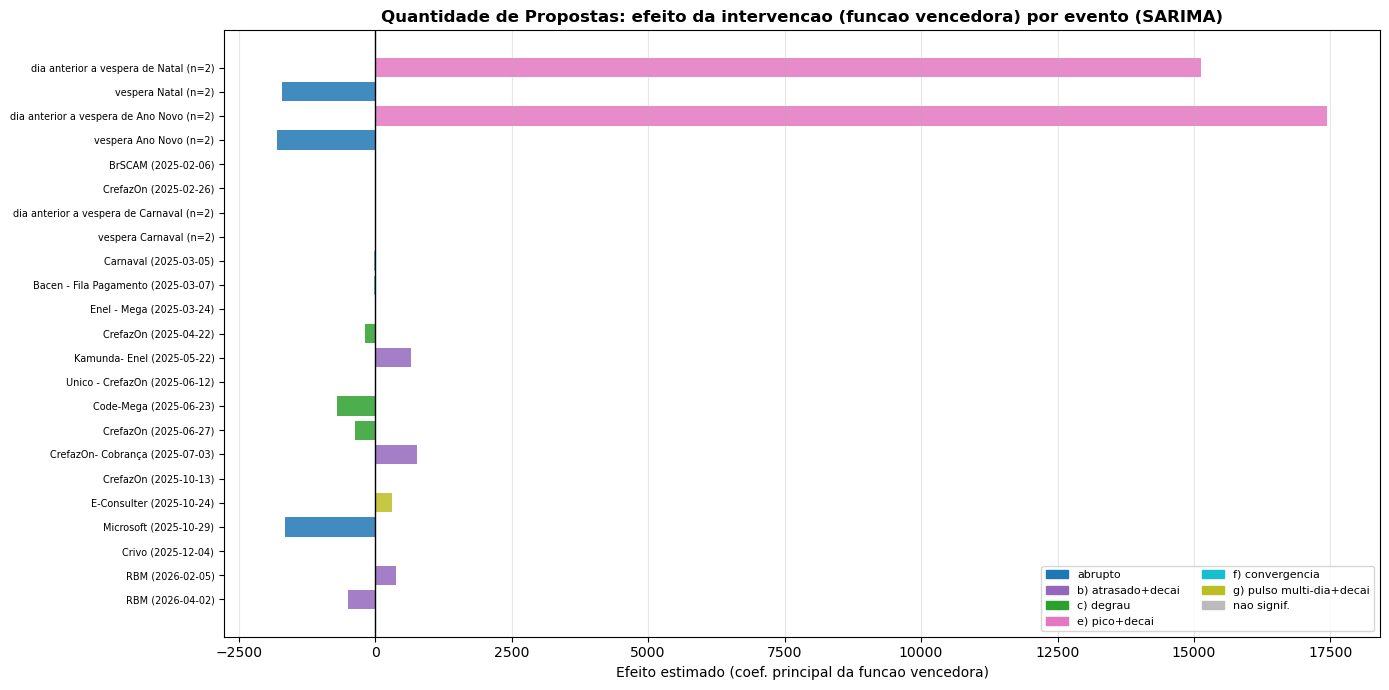
\includegraphics[width=0.99\linewidth]{interv_mag_qtd.png}
\caption{Magnitude do efeito estimado (coeficiente principal da função vencedora) por evento, para
o \textbf{valor} (topo) e a \textbf{quantidade} (base); a cor indica a forma de intervenção
vencedora. Os efeitos são predominantemente negativos (paradas derrubam a série); as vésperas de
Natal/Ano-Novo têm forte componente de cauda (função \emph{e}), e vários incidentes que pesam no
valor são \emph{não signif.}\ na quantidade.}
\label{fig:interv}
\end{figure}

\begin{figure}[H]
\centering
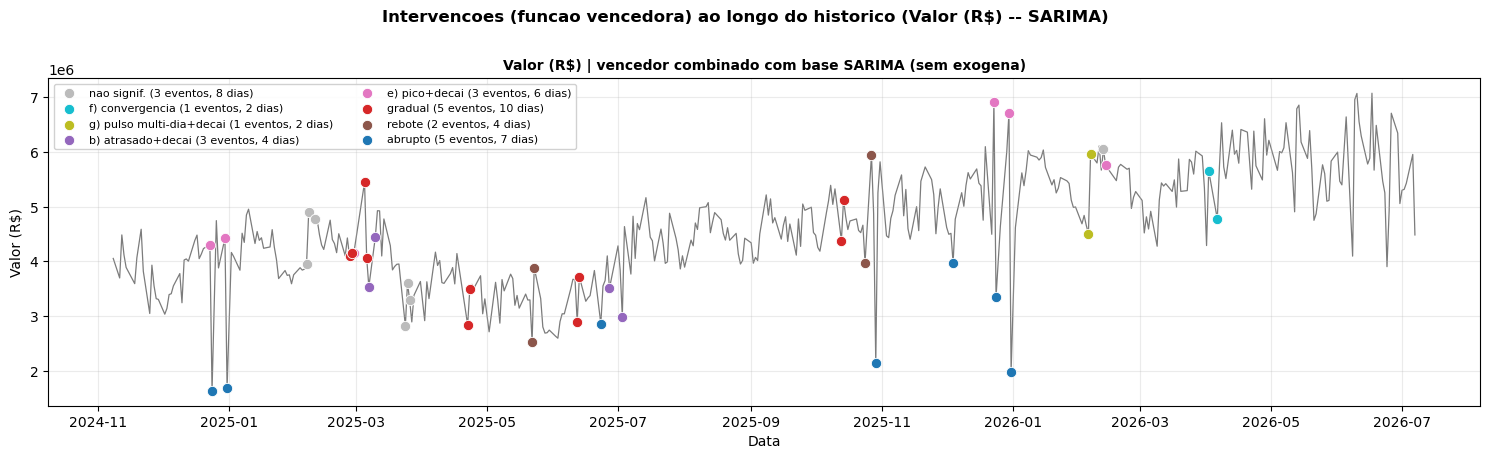
\includegraphics[width=0.99\linewidth]{interv_timeline_valor.png}\\[3pt]
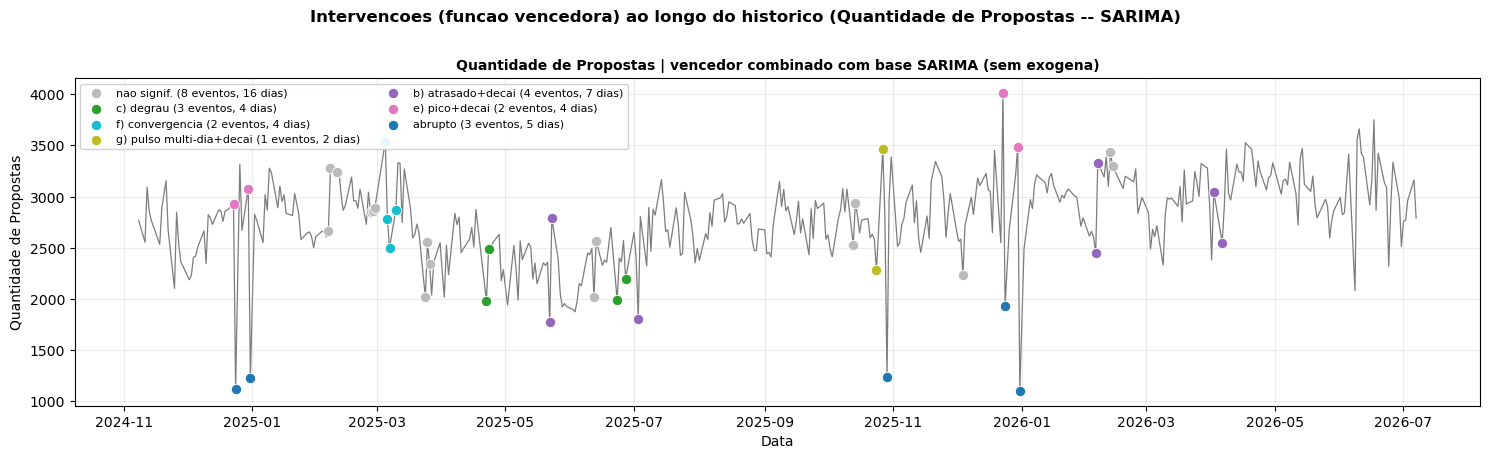
\includegraphics[width=0.99\linewidth]{interv_timeline_qtd.png}
\caption{Eventos de intervenção ao longo do histórico, sobre as séries de valor (topo) e
quantidade (base). Cada ponto marca um dia de evento, colorido pela \textbf{função vencedora}
(mesmo código da Figura~\ref{fig:interv}); os pontos cinza (``não signif.'') foram testados e
descartados. Fonte: modelo congelado de produção.}
\label{fig:interv-timeline}
\end{figure}

O efeito da intervenção sobre a \emph{qualidade do ajuste} é um dos resultados centrais: com as
\emph{dummies}, o \textbf{Ljung--Box deixa de rejeitar} a hipótese de resíduos
não-autocorrelacionados --- o $p(10)$ sobe de $\approx 0{,}01$ (sem intervenção, em ambas as
séries) para \textbf{0,37} (valor) e \textbf{0,63} (quantidade), como mostra a
Tabela~\ref{tab:coef}. Isso fica visual de duas formas. \textbf{(i) No tempo}: o resíduo \emph{pré}
intervenção tem \emph{spikes} enormes exatamente nos dias de \texttt{Log\_Erro} e véspera
(linhas marcadas); \emph{pós} intervenção esses picos desaparecem e o resíduo fica homogêneo
(Figuras~\ref{fig:resid-valor} e~\ref{fig:resid-qtd}). \textbf{(ii) Na distribuição}: no
\texttt{plot\_diagnostics} (Figuras~\ref{fig:diag-valor} e~\ref{fig:diag-qtd}), antes da
intervenção o \textbf{Q--Q} exibe uma cauda inferior pesada e o \textbf{histograma} é
leptocúrtico; depois, os resíduos se aproximam nitidamente da normal. Persistem, como ressalva,
\textbf{heterocedasticidade} e \textbf{caudas pesadas} residuais (Jarque--Bera significativo) ---
erros maiores nos dias atípicos ---, o que torna os intervalos de confiança otimistas nos extremos.

\begin{figure}[H]
\centering
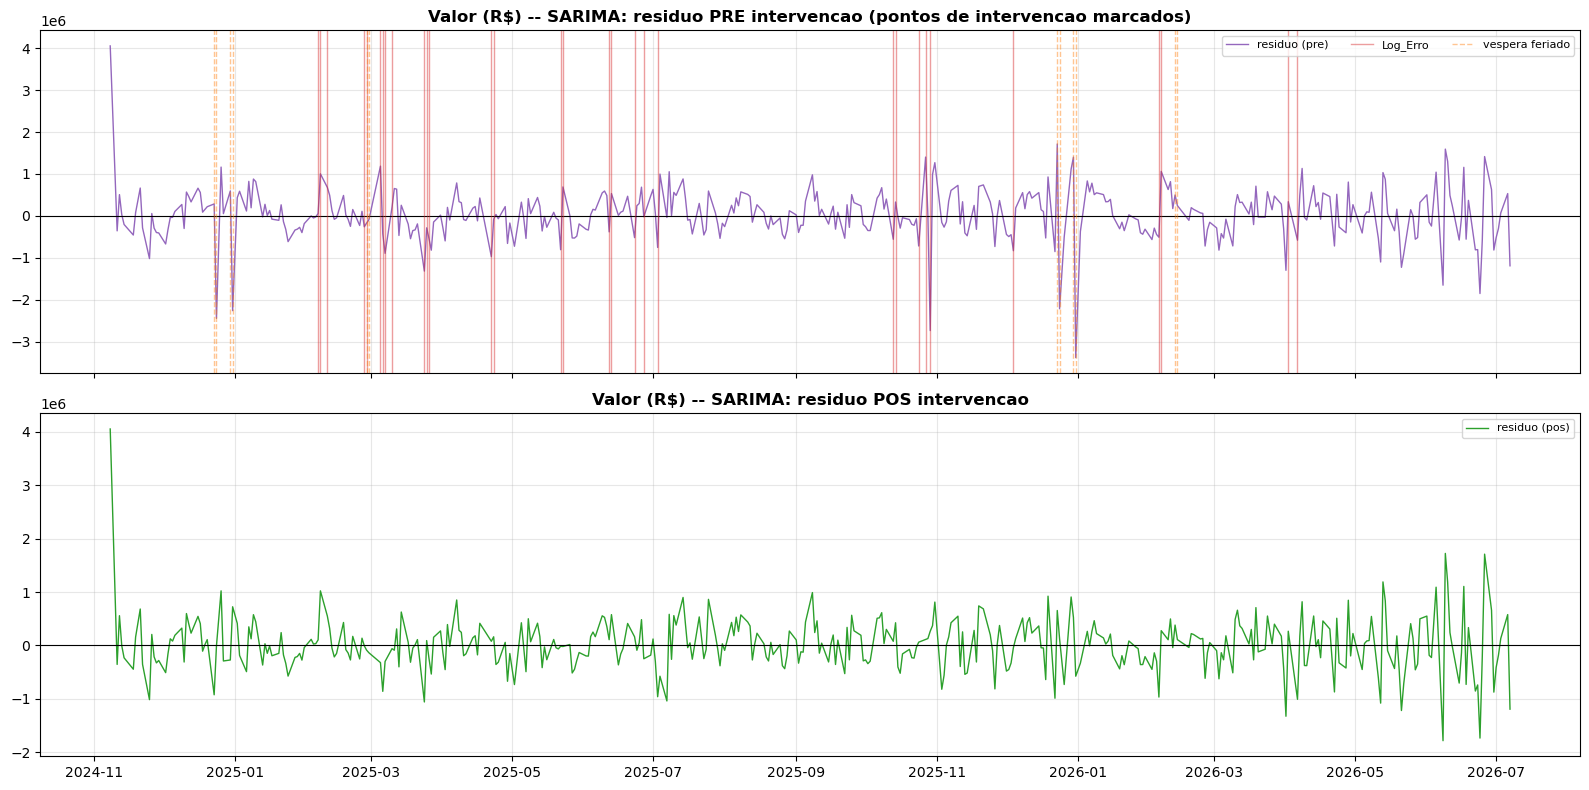
\includegraphics[width=0.98\linewidth]{interv_resid_valor.png}
\caption{Resíduo do SARIMA de \textbf{valor} ao longo do tempo, \emph{pré} (topo, com os dias de
\texttt{Log\_Erro} e véspera marcados) vs.\ \emph{pós} intervenção (base). Os \emph{spikes} nos
dias atípicos somem após o tratamento.}
\label{fig:resid-valor}
\end{figure}

\begin{figure}[H]
\centering
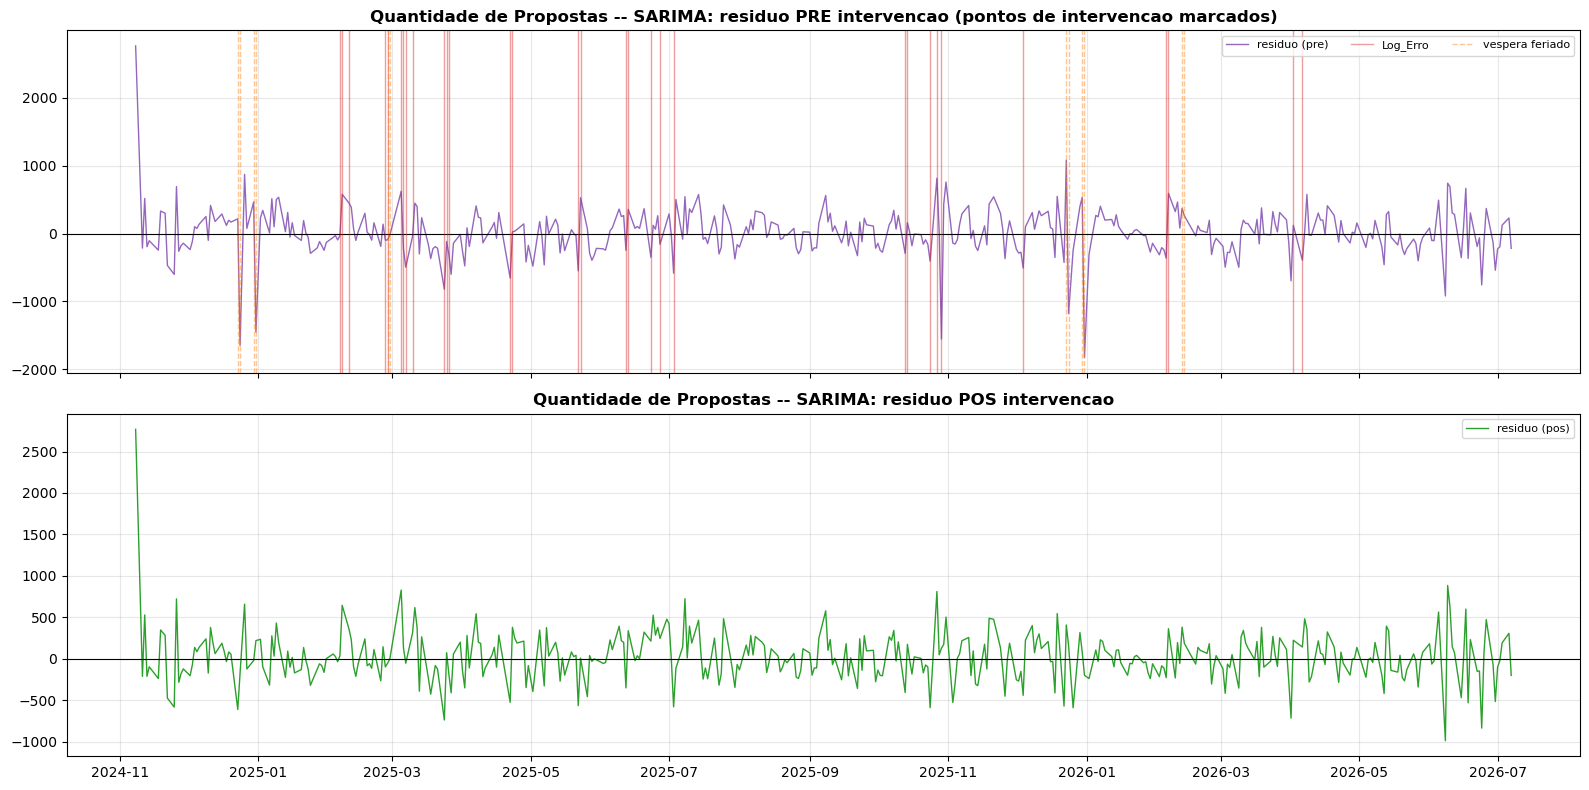
\includegraphics[width=0.98\linewidth]{interv_resid_qtd.png}
\caption{Resíduo do SARIMA de \textbf{quantidade} ao longo do tempo, \emph{pré} vs.\ \emph{pós}
intervenção. Mesmo efeito: os picos dos dias atípicos são absorvidos.}
\label{fig:resid-qtd}
\end{figure}

\begin{figure}[H]
\centering
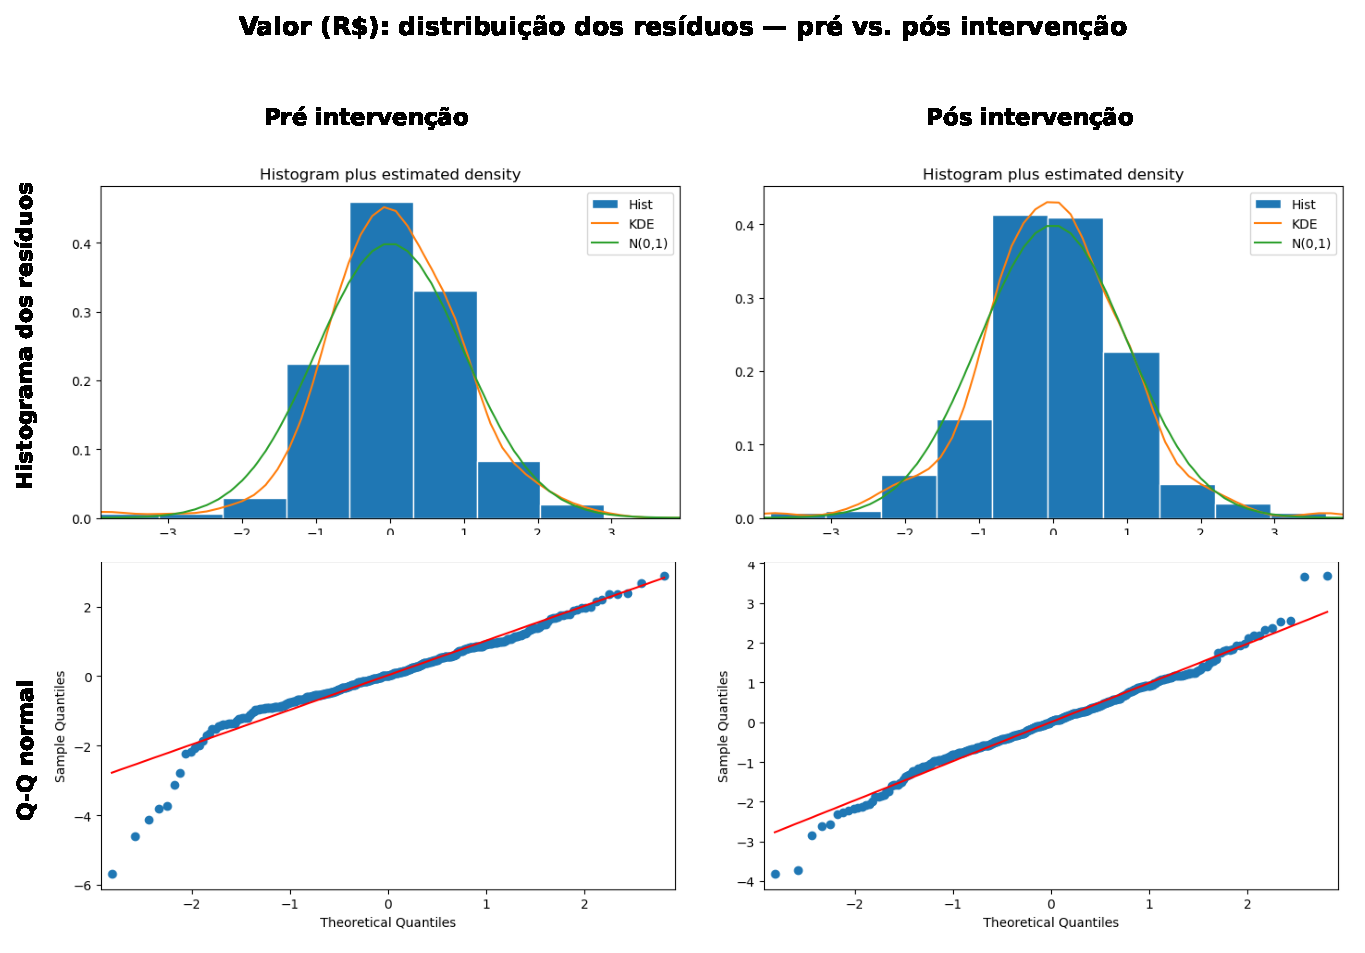
\includegraphics[width=0.95\linewidth]{diag_dist_valor.pdf}
\caption{Distribuição dos resíduos do SARIMA de \textbf{valor} --- histograma (topo) e Q--Q normal
(base), \emph{pré} (esquerda) vs.\ \emph{pós} (direita) intervenção. A cauda inferior pesada do
Q--Q (dias de erro puxando os resíduos) some após a intervenção, e o histograma se aproxima da
$N(0,1)$.}
\label{fig:diag-valor}
\end{figure}

\begin{figure}[H]
\centering
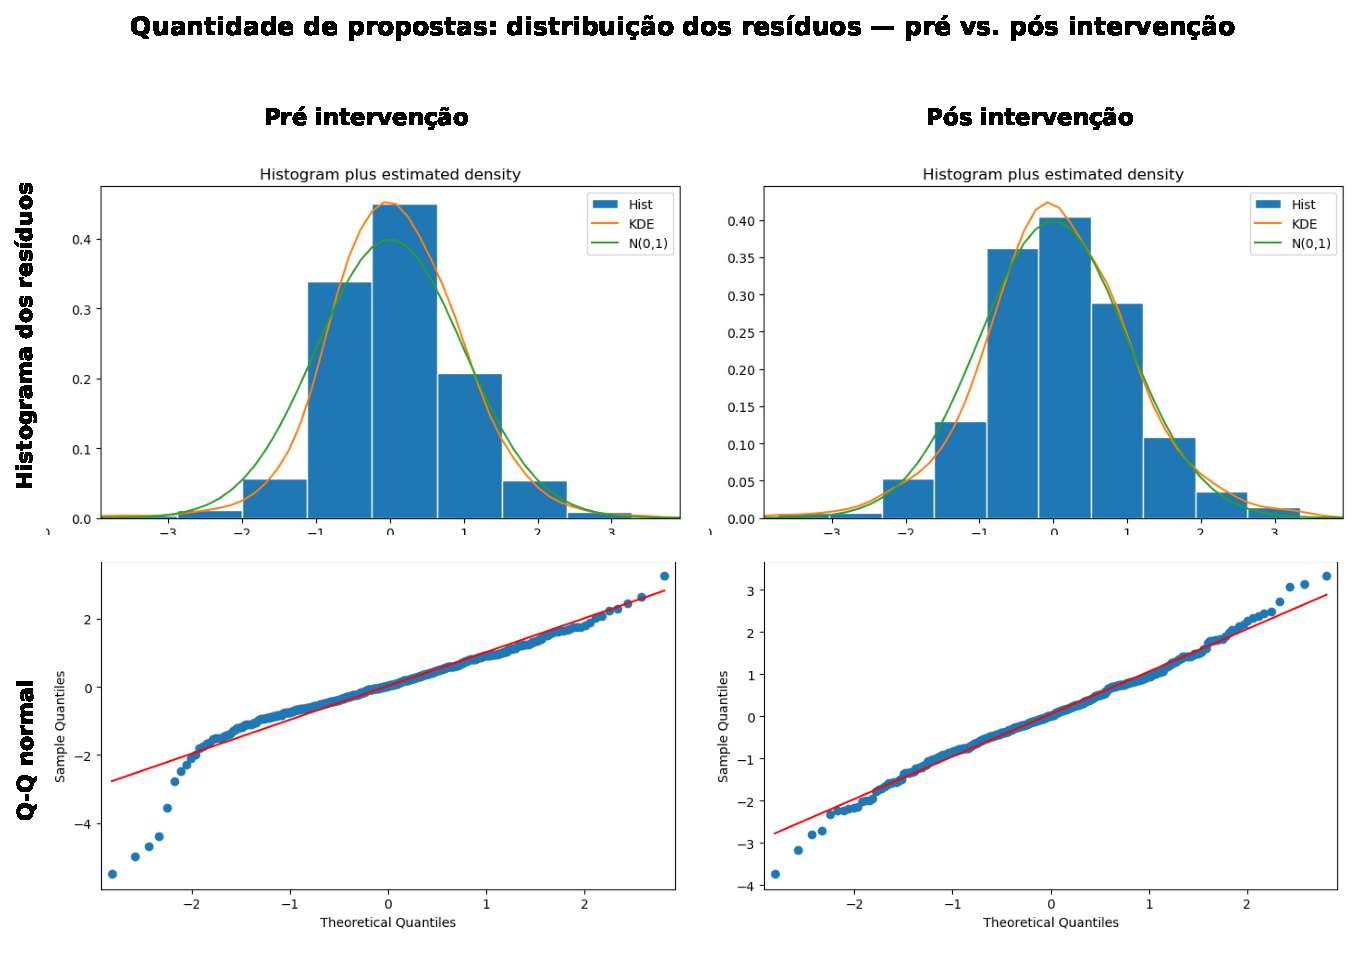
\includegraphics[width=0.95\linewidth]{diag_dist_qtd.pdf}
\caption{Distribuição dos resíduos do SARIMA de \textbf{quantidade} --- histograma (topo) e Q--Q
normal (base), \emph{pré} vs.\ \emph{pós} intervenção. Mesmo padrão: os resíduos se aproximam da
normal após tratar os dias atípicos.}
\label{fig:diag-qtd}
\end{figure}

\subsection{Estimação: coeficientes e significância}
\label{sec:res-est}

A Tabela~\ref{tab:coef} traz o ajuste \emph{in-sample} do modelo congelado (regressão com erros
SARIMA $+$ intervenção, $N=414$). O achado central é econométrico: o \textbf{motor preditivo é a
MA(1)}, não a sazonalidade. O termo $\theta_1 \approx -0{,}6$ é grande e altamente significativo
($p<0{,}001$) nas duas séries --- de longe o coeficiente mais forte. Num IMA(1,1), isso equivale a
uma \textbf{suavização do tipo média móvel exponencial}: a previsão de amanhã é o nível de hoje
corrigido por $\approx 60\%$ do erro de previsão de ontem. A \textbf{sazonalidade semanal é real,
mas fraca} ($\Theta$ pequenos e não significativos individualmente, $p\ge 0{,}11$): a maior parte
do padrão semanal já é absorvida pela diferenciação e pela grade de dias úteis.

\begin{table}[H]
\centering
\caption{Coeficientes \emph{in-sample} do modelo congelado ($N=414$ dias úteis) e diagnóstico de
Ljung--Box. Fonte: \texttt{docs/modelo\_sarima\_intervencoes.md}.}
\label{tab:coef}
\small
\begin{tabular}{@{}lcc@{}}
\toprule
Termo & \textbf{Valor} $(0,1,1)(0,0,1)_5$ & \textbf{Qtd} $(0,1,1)(0,0,2)_5$ \\
\midrule
MA(1) --- $\theta_1$ (choque de ontem) & $\mathbf{-0{,}645}$ · $p<0{,}001$ & $\mathbf{-0{,}605}$ · $p<0{,}001$ \\
MA sazonal --- $\Theta_1$ (lag 5)      & $-0{,}074$ · $p=0{,}11$ & $-0{,}035$ · $p=0{,}47$ \\
MA sazonal --- $\Theta_2$ (lag 10)     & --- & $+0{,}014$ · $p=0{,}79$ \\
AIC                                    & 11.796,7 & 5.661,2 \\
Ljung--Box $p(10)$ (com interv.)       & \textbf{0,37} \checkmark & \textbf{0,63} \checkmark \\
Ljung--Box $p(10)$ (sem interv.)       & $\approx 0{,}01$ \ding{55} & $\approx 0{,}01$ \ding{55} \\
\bottomrule
\end{tabular}
\end{table}

\subsection{\emph{Ranking} diário --- histórico completo}
\label{sec:res-rank}

Sob o mesmo protocolo \emph{walk-forward}, o SARIMA compete com a pipeline antiga e com os melhores
modelos de ML/TPOT. Os resultados diferem entre as séries e merecem leitura cuidadosa.

\paragraph{Valor (Tabela~\ref{tab:rank-valor}).} O SARIMA é o \textbf{1\textsuperscript{o}
colocado}: melhor RMSPE (9,36\%), melhor $R^2$ (0,750), menor viés (praticamente zero: $-594$ vs.\
$+29.991$ da antiga) e menor erro máximo (30,52\% vs.\ 39,52\%). Perde por pouco no MAPE médio para
a antiga (7,35\% vs.\ 7,19\%). É uma vitória limpa, e com viés quase nulo.

\begin{table}[H]
\centering
\caption{\emph{Ranking} --- Valor (histórico completo, ordenado por RMSPE). Viés e DP Erro em R\$.}
\label{tab:rank-valor}
\small
\setlength{\tabcolsep}{4.5pt}
\begin{tabular}{@{}lccccccc@{}}
\toprule
Modelo & MAPE\% & RMSPE\% & $R^2$ & Viés & Máx.\% & $<$10\% \\
\midrule
\textbf{SARIMA}                & 7,35 & \textbf{9,36} & \textbf{0,750} & \textbf{$-$594}   & \textbf{30,52} & 152/209 \\
Pipeline Antiga em Produção    & \textbf{7,19} & 9,54 & 0,748 & $+$29.991 & 39,52 & 156/211 \\
ExtraTrees (EXT, j90)          & 7,20 & 9,61 & 0,720 & $+$79.401 & 42,56 & \textbf{164/209} \\
POLY+ABR                       & 8,12 & 10,33 & 0,684 & $+$113.975 & 32,44 & 144/209 \\
Voting (GBR+XGB+RFR)           & 7,97 & 10,65 & 0,660 & $+$134.676 & 33,35 & 146/209 \\
\bottomrule
\end{tabular}
\end{table}

\paragraph{Quantidade (Tabela~\ref{tab:rank-qtd}).} Aqui a leitura é \emph{mista} e o relatório é
honesto quanto a isso. O SARIMA tem o \textbf{melhor MAPE médio (7,19\%)}, o \textbf{menor viés
(22,6)} --- centradíssimo --- e o \textbf{maior número de dias muito bons} (97/211 com erro
$<5\%$). Porém, no critério de \emph{ranking} (RMSPE) fica em 4\textsuperscript{o} (9,64\% vs.\
9,49\% do melhor ML) e tem o \textbf{pior erro máximo} (50,71\%): um único dia muito ruim
(justamente o que o RMSPE penaliza). Ou seja, o SARIMA é o \emph{mais bem centrado}, mas não o de
menor dispersão de cauda na quantidade --- ainda assim supera a pipeline antiga em RMSPE (9,64 vs.\
9,88) e em MAPE.

\begin{table}[H]
\centering
\caption{\emph{Ranking} --- Quantidade (histórico completo, $N=211$, ordenado por RMSPE).}
\label{tab:rank-qtd}
\small
\setlength{\tabcolsep}{4.5pt}
\begin{tabular}{@{}lcccccc@{}}
\toprule
Modelo & MAPE\% & RMSPE\% & $R^2$ & Viés & Máx.\% & $<$5\% \\
\midrule
SE(LINE)+SE(SGDR)+ABR          & 7,41 & \textbf{9,49} & 0,345 & 59,6 & 31,26 & 88 \\
SPct+ABR                       & 7,47 & 9,59 & 0,336 & 61,0 & 31,26 & 85 \\
SE(ABR)+MAS+OHE+ABR            & 7,32 & 9,62 & 0,328 & 43,7 & 34,42 & 96 \\
\textbf{SARIMA}                & \textbf{7,19} & 9,64 & 0,339 & \textbf{22,6} & 50,71 & \textbf{97} \\
SE(ETR)+MMS+BIN+SE(ELAS)+ABR   & 7,67 & 9,73 & 0,311 & 69,9 & 29,60 & 85 \\
Pipeline Antiga em Produção    & 7,89 & 9,88 & 0,313 & 40,5 & 34,06 & 87 \\
\bottomrule
\end{tabular}
\end{table}

No \textbf{recorte recente (janeiro em diante)} a vantagem dos modelos brancos cresce e fica mais
estável. O acompanhamento do previsto $\times$ realizado (Figura~\ref{fig:predreal}) mostra que o
SARIMA segue bem nível e sazonalidade, com os maiores erros nos saltos pós-atípicos --- onde a
pipeline antiga também erra.

\begin{figure}[H]
\centering
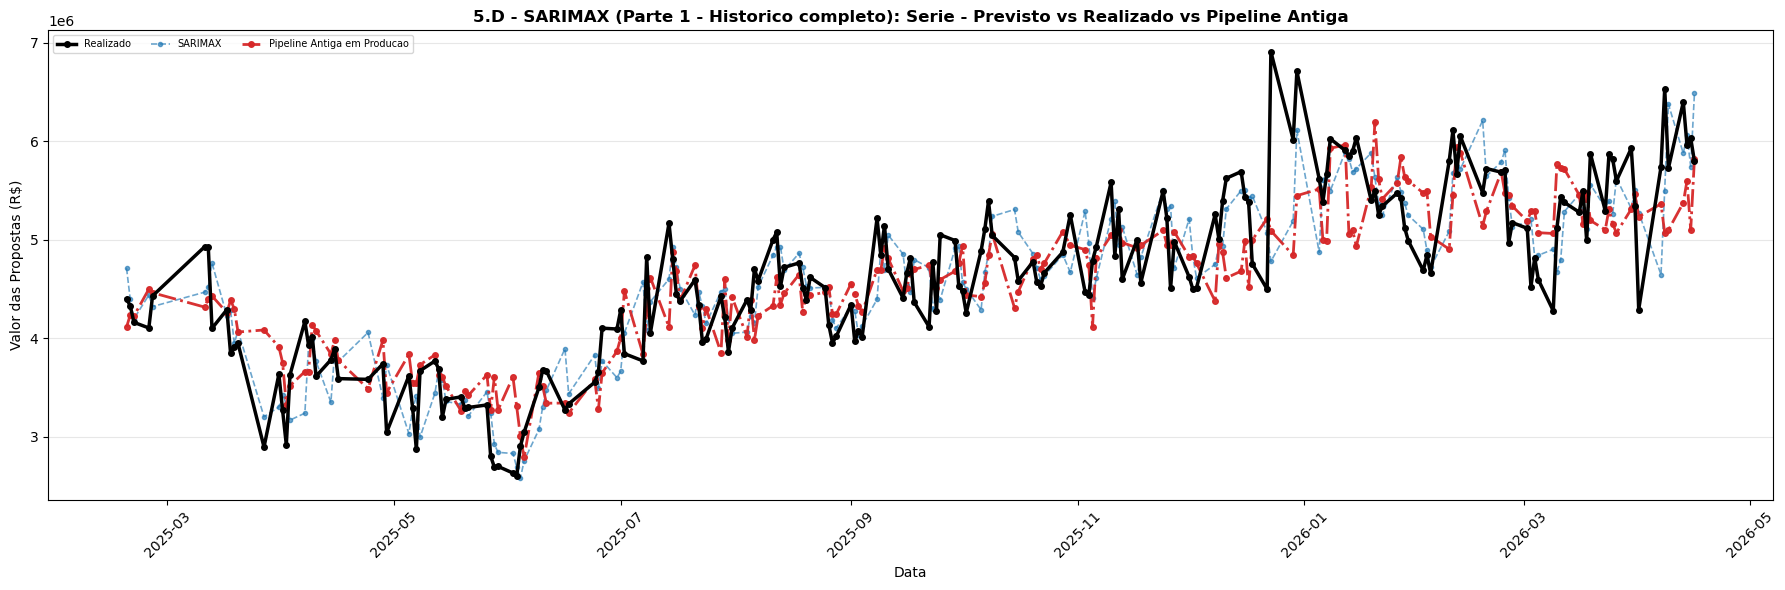
\includegraphics[width=0.9\linewidth]{valor_pred_real.png}
\caption{Valor previsto (SARIMA) $\times$ realizado $\times$ pipeline antiga ao longo do período de
avaliação. Os maiores erros concentram-se nos saltos pós-atípicos.}
\label{fig:predreal}
\end{figure}

\subsection{Modelos mensais: \emph{nowcast} e comparação}
\label{sec:res-nowcast}

Como extensão, estuda-se a previsão do \textbf{total do mês}. O \emph{nowcast} soma o realizado
acumulado até o dia $D$ à previsão SARIMA dos dias úteis restantes:
$\text{Nowcast}(D) = \text{acumulado}(\le D) + \widehat{\text{restante}}$; conforme o mês avança,
mais dias viram realizado e a estimativa converge (Figura~\ref{fig:nowcast}). Agregando os 19 meses
completos, o $|\text{Erro }\%|$ mediano começa em $\approx 5$--$7\%$ e cai para $<2\%$ a partir de
$\approx 2/3$ do mês.

Comparando abordagens de total mensal (Tabelas~\ref{tab:mensal-valor} e~\ref{tab:mensal-qtd}),
\textbf{um resultado honesto se impõe}: para o total mensal, a \emph{persistência} ingênua
(\textbf{Naive}, repetir o mês anterior) é a melhor, e o modelo paramétrico direto (ARIMAX) é o
\emph{pior}. O nowcast fica em posição intermediária --- útil por atualizar em tempo real ao longo
do mês, mas não a melhor previsão \emph{a priori} do total.

\begin{table}[H]
\centering
\caption{Total mensal --- \textbf{Valor}. Ordenado por RMSPE. (Viés em R\$.)}
\label{tab:mensal-valor}
\small
\begin{tabular}{@{}lcccccc@{}}
\toprule
Modelo & MAPE\% & RMSPE\% & Mediana\% & Máx.\% & $R^2$ \\
\midrule
\textbf{Naive (mês$-1$)}       & \textbf{3,53} & \textbf{4,66} & 2,33 & \textbf{9,50} & \textbf{0,641} \\
Nowcast (últ.\ dia mês$-1$)    & 4,43 & 5,27 & 4,17 & 11,04 & 0,547 \\
MediaUtil MM3                  & 6,17 & 6,92 & 5,29 & 11,80 & 0,280 \\
ARIMAX                         & 7,70 & 8,53 & 7,77 & 14,18 & $-0{,}078$ \\
\bottomrule
\end{tabular}
\end{table}

\begin{table}[H]
\centering
\caption{Total mensal --- \textbf{Quantidade}. Ordenado por RMSPE.}
\label{tab:mensal-qtd}
\small
\begin{tabular}{@{}lcccccc@{}}
\toprule
Modelo & MAPE\% & RMSPE\% & Mediana\% & Máx.\% & $R^2$ \\
\midrule
\textbf{Naive (mês$-1$)}       & \textbf{2,94} & \textbf{3,64} & 2,80 & \textbf{6,89} & \textbf{0,597} \\
MediaUtil MM3                  & 3,27 & 4,06 & 2,77 & 7,19 & 0,519 \\
Nowcast (últ.\ dia mês$-1$)    & 4,19 & 4,57 & 3,82 & 7,80 & 0,368 \\
ARIMAX                         & 5,49 & 6,55 & 3,65 & 11,17 & $-0{,}277$ \\
\bottomrule
\end{tabular}
\end{table}

\begin{figure}[H]
\centering
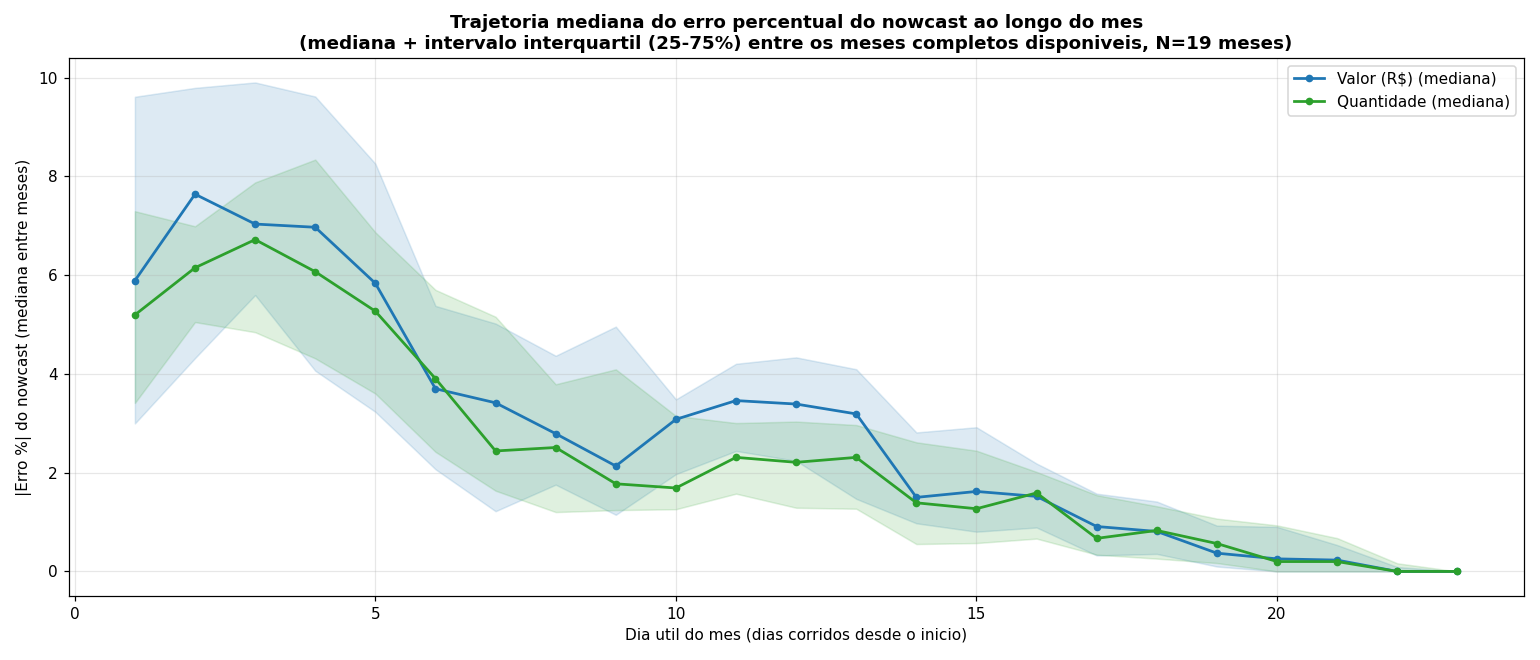
\includegraphics[width=0.8\linewidth]{nowcast_trajetoria_erro.png}
\caption{Trajetória mediana do erro percentual do \emph{nowcast} ao longo do mês (faixa: IQR
25--75\% entre meses), valor e quantidade.}
\label{fig:nowcast}
\end{figure}

%========================================================================
\section{Discussão e interpretação}
\label{sec:disc}

Os modelos revelam, com significância estatística:
\begin{enumerate}\setlength\itemsep{2pt}
\item \textbf{As séries têm nível que passeia}, não uma média fixa ($I(1)$): a melhor âncora para
amanhã é o nível de hoje, não uma média histórica.
\item \textbf{O motor é a MA(1)}, não a sazonalidade: $\theta_1\approx-0{,}6$ ($p<0{,}001$) domina;
o padrão semanal é real mas fraco.
\item \textbf{Dias de erro têm efeito real e mensurável} --- entram como \emph{intervenção}, não
como descarte. Muitos afetam o \emph{valor} sem afetar a \emph{quantidade} (8/23 ``não signif.'' na
qtd), e o efeito tipicamente tem cauda (\emph{backlog}).
\item \textbf{Valor e quantidade não compartilham equilíbrio de longo prazo} --- a modelagem
separada é a escolha correta.
\end{enumerate}

\paragraph{Leitura crítica.} O argumento a favor do modelo branco é \textbf{forte no valor}
(SARIMA 1\textsuperscript{o} em RMSPE, $R^2$, viés e erro máximo) e \textbf{qualitativamente forte
nas duas séries} (interpretabilidade, diagnóstico de Ljung--Box, especificação congelada). Deve-se
ser honesto, porém, em dois pontos: (i) na \textbf{quantidade}, o SARIMA \emph{não} é o melhor no
critério de \emph{ranking} (RMSPE 9,64\%, 4\textsuperscript{o}) e tem o \emph{pior} erro máximo
(50,71\%) --- é o mais bem centrado (menor viés, melhor MAPE), mas paga em um dia de cauda; (ii) o
\textbf{ganho de acurácia} sobre a pipeline antiga é, no geral, \emph{marginal}. A tese que se
sustenta com robustez não é ``prevê muito melhor'', e sim ``\textbf{empata ou supera em acurácia e
ganha em interpretabilidade, auditabilidade e tratamento explícito de choques}'', com a vantagem
operacional de uma \emph{única} especificação congelada contra o retreino diário da caixa-preta.
Nos \textbf{totais mensais}, a recomendação prática é a persistência (Naive)/nowcast, não o
paramétrico direto.

%========================================================================
\section{Conclusão}
\label{sec:conc}

\begin{itemize}\setlength\itemsep{2pt}
\item \textbf{Valor} $\to$ SARIMA $(0,1,1)(0,0,1)_5 +$ intervenção: 1\textsuperscript{o} no
\emph{ranking}, melhor RMSPE (9,36\%), $R^2$ (0,750) e viés quase nulo.
\item \textbf{Quantidade} $\to$ SARIMA $(0,1,1)(0,0,2)_5 +$ intervenção: melhor MAPE e viés,
supera a pipeline antiga em RMSPE; univariado e parcimonioso.
\end{itemize}

\noindent
Responde-se afirmativamente à pergunta de pesquisa: um modelo \emph{branco}, com especificação
única congelada, \textbf{iguala ou supera} a pipeline em produção nas duas séries, sem abrir mão de
interpretabilidade. A análise de intervenção de Box--Tiao mostrou-se decisiva para descontaminar o
ajuste (Ljung--Box de $\approx 0{,}01$ para 0,37/0,63) e a ausência de cointegração legitimou a
modelagem separada --- confirmada pelo teste de limites \textbf{ARDL} (que também não rejeita a
ausência de relação de nível) e, empiricamente, pelo \emph{walk-forward}, já que nenhuma alternativa
conjunta (ticket, ARDL, SUR ou VAR) supera o SARIMA univariado (Tabela~\ref{tab:joint}). Em uma
frase: \emph{ambas as séries são bem descritas por uma suavização MA(1) sobre a série diferenciada,
com sazonalidade semanal leve e os dias atípicos tratados explicitamente por intervenção de
Box--Tiao}.

\paragraph{Limitações e próximos passos.} (i) \textbf{Heterocedasticidade e caudas pesadas} nos
resíduos tornam os intervalos de confiança otimistas nos extremos --- modelar a variância
(\textbf{GARCH}) daria IC honestos também para os dias típicos; (ii) a modelagem \emph{conjunta}
poderia ainda ser explorada por um \textbf{modelo de fator dinâmico} ou por SUR com covariância de
erro plena (útil para \emph{intervalos conjuntos}, ainda que sem ganho de ponto esperado, dado o elo
contemporâneo); (iii) validar e aprimorar os \textbf{modelos mensais} (o Naive vencer sugere reavaliar o nowcast
como acompanhamento, não como previsão \emph{a priori}); (iv) a classe da intervenção é fixada uma
vez na série inteira (\emph{look-ahead} estrutural leve, mitigado por ser majoritariamente
calendário).

%========================================================================
\section*{Referências}
\addcontentsline{toc}{section}{Referências}
\small
\begin{itemize}
\item Box, G.\,E.\,P.; Jenkins, G.\,M.; Reinsel, G.\,C. \emph{Time Series Analysis: Forecasting and
Control}. Wiley.
\item Box, G.\,E.\,P.; Tiao, G.\,C. (1975). \emph{Intervention Analysis with Applications to
Economic and Environmental Problems}. JASA, 70(349), 70--79.
\item Engle, R.\,F.; Granger, C.\,W.\,J. (1987). \emph{Co-integration and Error Correction}.
Econometrica, 55(2), 251--276.
\item Johansen, S. (1991). \emph{Estimation and Hypothesis Testing of Cointegration Vectors in
Gaussian VAR Models}. Econometrica, 59(6), 1551--1580.
\item Pesaran, M.\,H.; Shin, Y.; Smith, R.\,J. (2001). \emph{Bounds Testing Approaches to the
Analysis of Level Relationships}. J.\ Applied Econometrics, 16(3), 289--326.
\item Apresentação de referência: \emph{Projeção de Vendas --- Definição de Modelo (v2)}.
\item Documentação interna do projeto: \path{docs/apresentacao_sarima_valor.md},
\path{docs/modelo_sarima_intervencoes.md}, \path{config/modelo_sarima_producao.json}.
\end{itemize}

\end{document}
